\subsubsection{Motivations}

Till this point, we have discussed extensively on the theoretical approaches that enables us to determine the energetic stabilities and physical properties of materials, starting from their chemical compositions and atomistic structures, which constitute a forward mathematical mapping of $\{\mathcal{C},\bm{R}\}\xrightarrow{f}\{\mathcal{P}\}$. However, the ultimate goal in the computer-guided materials discoveries, is to inversely design new materials\cite{zunger2018inverse} that aims to propose/sample the compositions and structures of new materials that possess certain properties, or to be  mathematically formulated as to solve and develop an inverse mapping of   $\{\mathcal{P}\}\xrightarrow{f^{-1}}\{\mathcal{C},\bm{R}\}$. As NN has shown its unique capability as a universal approximator for solving the forward mapping problem $\mathcal{P}=f_{\boldsymbol{\theta}}(\mathcal{C},\bm{R})$, which, in principle, can also be trained to realise a model that approximate the inverse mapping of $(\mathcal{C},\bm{R})=f^{-1}_{\boldsymbol{\varphi}}(\mathcal{P})$. This motivates the development of generative AI methods for exploring new materials. 

Focusing further on the energetic stabilities $\mathcal{P}(\bm{R})=E(\bm{R})$ together with the data-driven and probabilistic perspective of AI models, the core problem that one would like to address in generative AI modelling can be formulated as following. Given the knowledge of a set of structures $\{\bm{R}\}$ that possess the stabilities $\{E\}$ is $p(\bm{R})$ (which, in this case, is the Boltzmann distribution), then can we directly draw new structures $\bm{R}_{\mathrm{new}}$ from $p(\bm{R})$, provided that we can somehow learn the highly complex probability distribution of $p(\bm{R})$ with a universal approximator, such as NN. Answering such a question leads to a fundamentally different, and conceptually broader, statistical sampling paradigm for exploring the materials space compared to traditional energy-based PES sampling approaches based on MD/MC [\cref{chapter:sampling_methods}]. 

Firstly, the bespoke generative model should, in principle, help to overcome the ergodicity challenge in statistical samplings that often require long time/Markov chain to discover rare minima separated by high energy barriers, thus leading to extremely low probabilities in discovering new structures. Secondly, whilst energy-based models strongly rely on the knowledge of gradient (or forces, $\nabla_{\bm{R}}E(\bm{R})$) to drive the sampling process to reach new local minima, in general, we do not necessarily know how to compute $\nabla_{\bm{R}}\mathcal{P}(\bm{R})$ with respect to any property of interest, particularly, in a broader context, the \emph{alchemical derivatives}\cite{anatole2009accurate,sheppard2010alchemical}   $\nabla_\mathcal{C}\mathcal{P}$ that informs us on how the property changes with respect to the change in the chemical compositions, that can be applied to guide our exploration of materials across the chemical space. The development of generative AI models for materials discoveries are posed to address these challenges.  

\subsubsection{Frameworks of Common Generative Models}
\label{sec:common_generative_models}

In this section, we shall provide a brief account on the architectures behind three most prominent generative models that have been applied to material and molecule discoveries in the past five years, namely, the variational autoencoders (VAE),\cite{kingma2013auto} the diffusion generative model\cite{sohl2015deep,song2019generative,song2020score,ho2020denoising} (which shares a close linkage with the hierarchical VAE\cite{sonderby2016ladder}), and finally the flow-based generative model.\cite{rezende2015variational} 

\begin{figure}[htb]
    \centering
    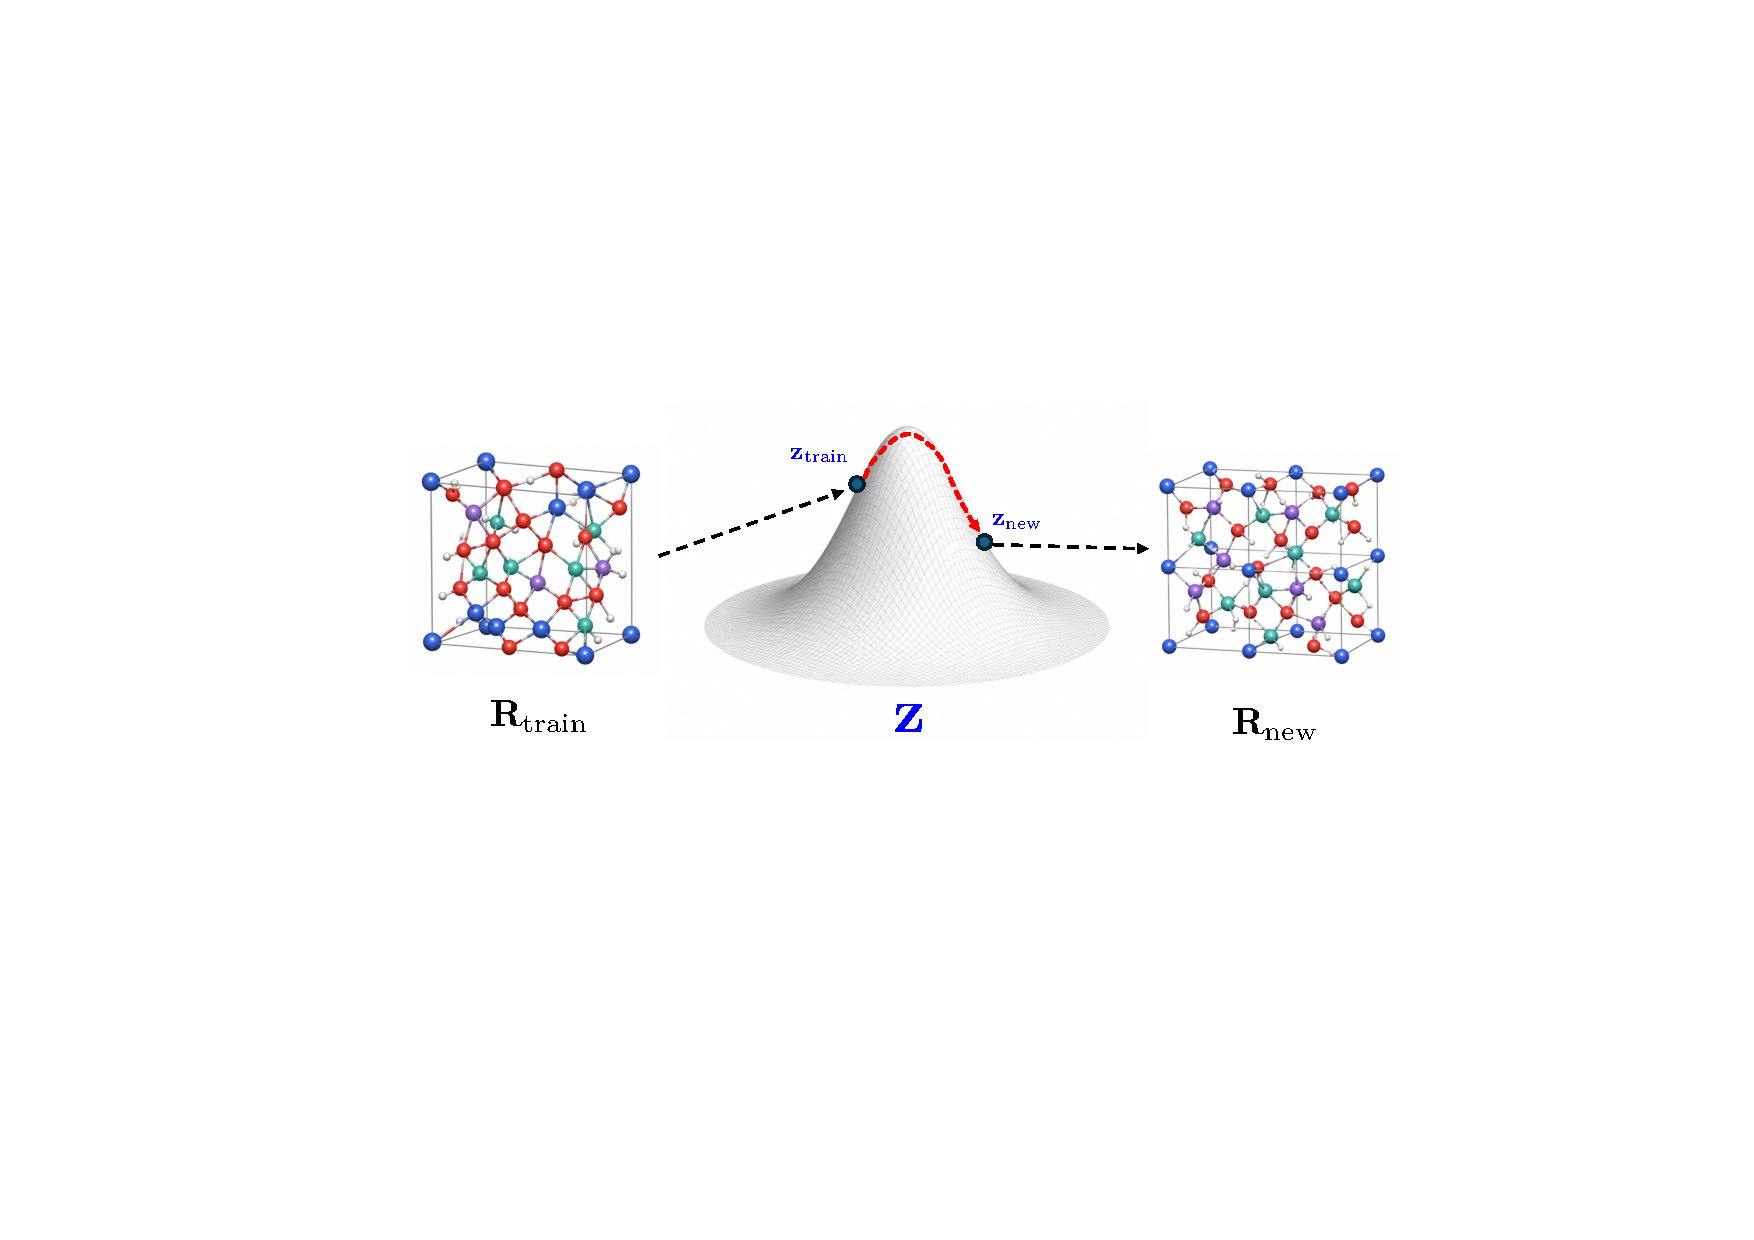
\includegraphics[width=0.7\linewidth]{generative_general_concept.pdf}
    \caption{General design concept behind modern generative AI models for materials discovery, which the training data $\bm{R}_{\mathrm{train}}$ that follows complex multimodal probability distribution is first converted into a latent variable $\bm{z}_{\mathrm{train}}$ that follows a simple, easy-to-sample distribution in the latent space. Subsequently, sampling a new latent variable $\bm{z}_{\mathrm{new}}$ in the latent space, and use it as the input in the inverse generative step will lead to a new material structure $\bm{R}_{\mathrm{new}}$. }
    \label{fig:generative_general_concept}
\end{figure}




In a high level overview (\cref{fig:generative_general_concept}), all these three generative models aims to overcome the problem of sampling complex multimodal probability distributions of $p(\bm{R})$ by first mapping the input/training structure $\bm{R}_{\mathrm{train}}\in \mathbb{R}^{3N}$ into a \emph{latent space} variable $\bm{z}_{\mathrm{train}}$, which may or may not be of a lower dimensionality of $\bm{R}_{\mathrm{train}}$, but most importantly, follow a simple probability distribution $p(\bm{z})$ that is easy to sample from, such as $p(\bm{z})\sim\mathcal{N}(\bm{z}|0,\bm{I})$. Providing that we can achieve the forward mapping by training a model $\bm{z}=f_{\boldsymbol{\varphi}}(\bm{R})$, and conjunctively learn a model that enables the inverse mapping $\bm{R}=g_{\boldsymbol{\theta}}(\bm{z})$, then, in principle, one could easy generate new samples $\bm{R}_{\mathrm{new}}$ by first sampling a new latent variable $\bm{z}_{\mathrm{new}}\sim p(\bm{z})$ (with negligible cost) followed by the application of the inverse mapping  $\bm{R}_{\mathrm{new}}=g_{\boldsymbol{\theta}}(\bm{z}_{\mathrm{new}})$.  



\begin{wrapfigure}[28]{rt}{0.5\textwidth}
  \begin{center}
    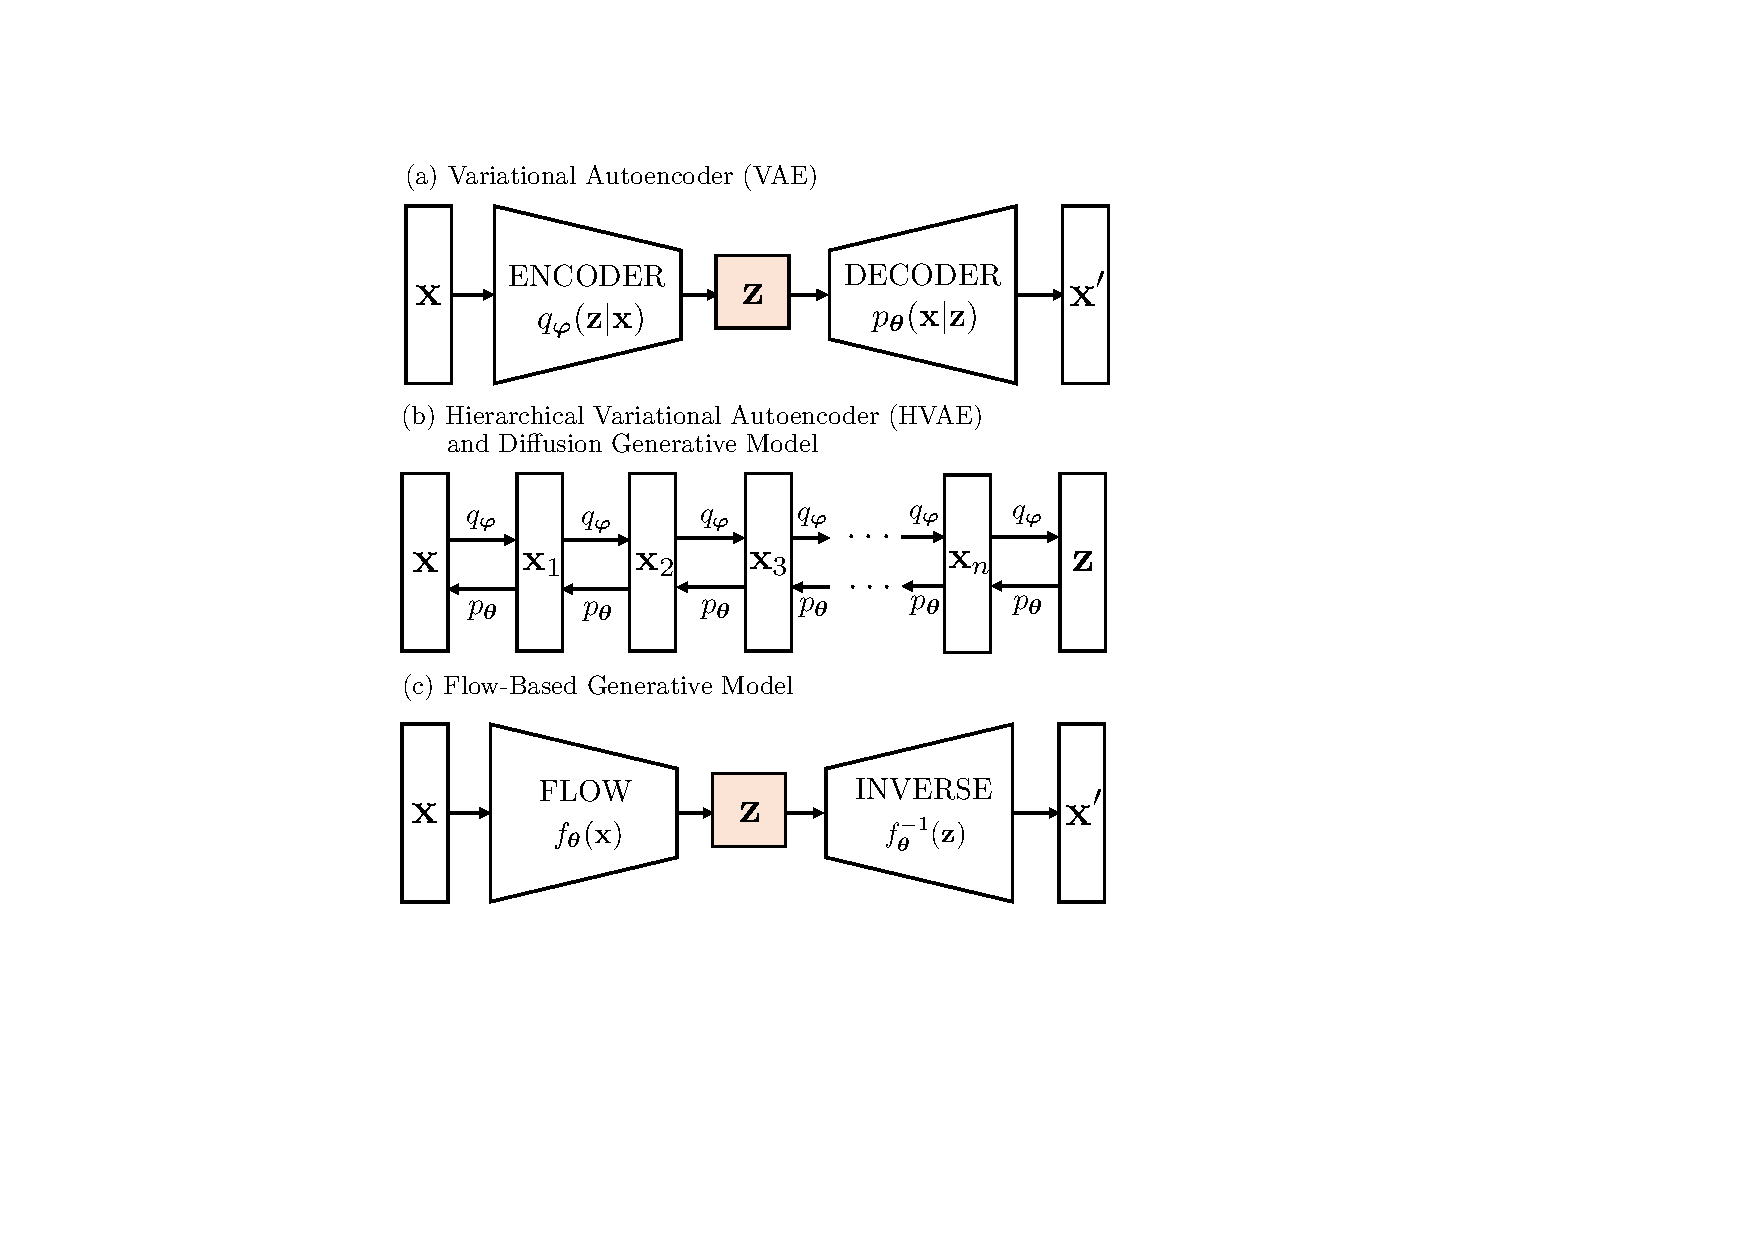
\includegraphics[width=0.5\textwidth]{generative_models.pdf}
    \caption{Schematic illustration of the architectures behind the three key generative models discussed in this work.}
    \label{fig:generative_models}
  \end{center}
\end{wrapfigure}


Without lost of generality, most modern structural generative models\cite{xie2021crystal,midgley2023se,zeni2025generative,kohler2019equivariant,klein2023equivariant}  tend to adopt equivariant NNs [\cref{sec:dl_fundamentals}] as the inductive bias to approximate the functions $\{f_{\boldsymbol{\varphi}},g_{\boldsymbol{\theta}}\}$ to achieve the efficient transformations between the real and latent space, such that we do not need to drill into the details of the NN architectures here but focusing more on the transformation process $\bm{x}\Leftrightarrow\bm{z}$ itself\footnote{In what follow, we shall be using $\bm{x}$ and $\bm{R}$ interchangeably to denote the inputs to the generative models.}. For the latter, we can further classify the transformations between $p(\bm{x})$ and $p(\bm{z})$ to be either achieved through an \emph{one-shot} (in VAE and flow-based models) or \textit{progressive} (in HVAE and diffusion models to enhance the quality of the generated models) procedure [\cref{fig:generative_models}], whereby the \textit{progressive} generative models would also enable us  \cite{song2019generative,song2020score} to apply techniques from stochastic differential equations to evolve the samples, in a way similar to the case of evolving structures on the PES with MD simulations while maintaining a desired thermodynamic ensemble through stochastically interacting with the thermo-/baro-stats (\cref{sect:molecular_dynamics}). Finally, building the foundation of probability interpretation of AI models, one could easily cast the problem of \emph{property-guided materials discovery} into the mathematical concepts of transforming between the  probabilities  of observing a specific structure/latent variable that is conditioned on the desired property, \emph{i.e.} $p(\bm{x}|\mathcal{P})\Leftrightarrow p(\bm{z}|\mathcal{P})$,\cite{ho2022classifier}  opening the implementable pathways to achieve property-driven inverse design of materials in modern atomistic materials simulations.


%\begin{figure}
%    \centering
%    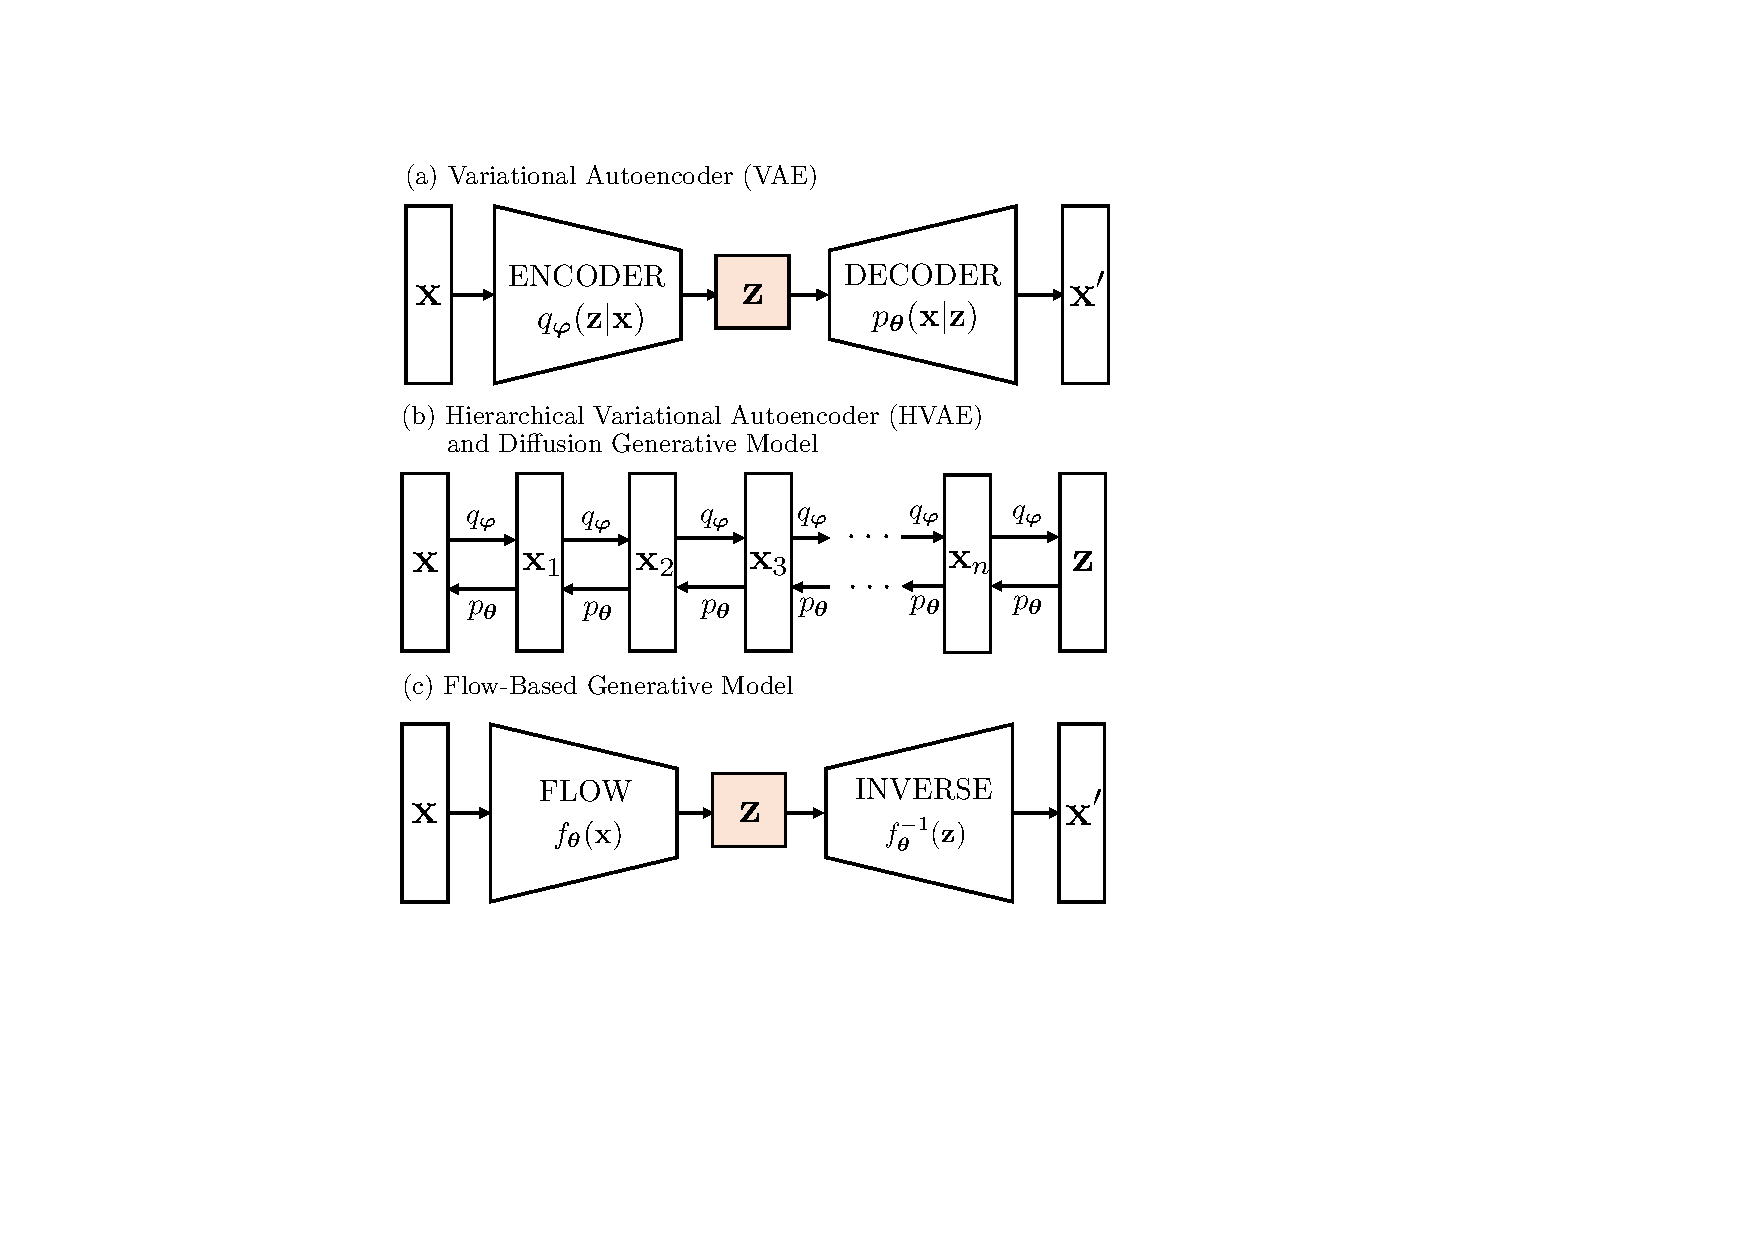
\includegraphics[width=0.5\linewidth]{generative_models.pdf}
%    \caption{Schematic illustration of the architectures behind the three key generative models discussed in this work.}
%    \label{fig:generative_models}
%\end{figure}

Conceptually, VAE [\cref{fig:generative_models}(a)] possesses a model architecture that is the easiest to understand, which largely follows the general conceptual frameworks for generative models discussed in the beginning.  Here, a forward NN is used to learn a map from the input $\bm{x}$ into the latent variable $\bm{z}$, or equivalently, the parameterised probability distribution of the latent variable conditioned on the input space $q_{\boldsymbol{\varphi}}(\bm{z}|\bm{x})$. This is to be combined with a backward NN that learns how to \emph{reconstruct} the real sample $\bm{x}$ from a given latent variable $\bm{z}$, which is in term governed by the conditional decoding distribution of $p_{\boldsymbol{\theta}}(\bm{x}|\bm{z})$. 

Denoting both model parameters collectively as $\boldsymbol{\phi}=(\boldsymbol{\varphi},\boldsymbol{\theta})$, training the generative model is similar to the training of supervised ML models (\cref{appendix:supervised_ML}) that aims to maximise the probability of observing the input samples over the parameter space, \emph{i.e.}
\begin{equation}
    \label{eq:argmax_phi_VAE}
    \hat{\boldsymbol{\phi}}=\argmax_{\boldsymbol{\phi}}p_{\boldsymbol{\phi}}(\bm{x}),
\end{equation}
whereby in VAE, $p(\bm{x})$ is obtained by marginalising the joint probability $p(\bm{x},\bm{z})$ over the latent space, \emph{i.e.} $p(\bm{x})=\int p(\bm{x},\bm{z})\mathrm{d} \bm{z}$. However, working directly with $p(\bm{x})$ is not mathematically tractable because in statistical thermodynamics, the full distribution $p(\bm{x})$ is normalised as $p=p^\prime/Z$ by the normalisation constant $Z=\int p^\prime(\bm{x})\mathrm{d}\bm{x}$ integrated over the full sample space, computing which thus requires a full configurational space sampling that satisfies the ergodic condition. This problem is commonly circumvented by taking the logarithm of the probability $\log p(\bm{x})=\log p^\prime(\bm{x})-\log Z$, which factors out a constant term of $\log Z$ that will not affect the outcome of the optimisation problem.\cite{sohl2015deep} This effectively cast the model optimisation problem of (\ref{eq:argmax_phi_VAE}) into a minimisation one as
\begin{equation}
    \label{eq:argmax_log_prob_phi_VAE}
    \hat{\boldsymbol{\phi}}=\argmin_{\boldsymbol{\phi}}[-\log p_{\boldsymbol{\phi}}(\bm{x})].
\end{equation}
The next problem to be solved is how to tackle the intractable joint probability distribution of $p(\bm{x},\bm{z})$. This is also easy to understand, as $p(\bm{z})$ is established with a trained NN model, hence it is not possible to compute $p(\bm{x},\bm{z})$ during the model training process. The trick here is to apply the Baye's rule followed by the Jansen's inequality (\cref{fig:generative_model_relations}) to derived an ELBO, which is to be used as the upper bound of the negative log-likelihood [\cref{eq:argmax_log_prob_phi_VAE}] in model training that will jointly optimised the parameters in both the encoder and decoder:\cite{luo2022understanding}
\begin{equation}
    \label{eq:VAE_ELBO}
    \mbox{ELBO}=\underbrace{ \mathbb{E}_{q_{\boldsymbol{\varphi}}(\bm{z}|\bm{x})}\left[p_{\boldsymbol{\theta}}(\bm{x}|\bm{z})\right]}_{\mbox{\scriptsize{reconstruction loss}}}
    -\underbrace{\mathcal{D}_{\mathrm{KL}}\left(  q_{\boldsymbol{\varphi}}(\bm{z}|\bm{x})||p(\bm{z}) \right)}_{\mbox{\scriptsize{prior matching}}}.
\end{equation}
Here, the reconstruction loss measures the averaged agreement between the input data and the latent variables, whereas the prior matching term measures how well the latent variables generated from the forward network follows the prior distribution of the latent variables. Minimising the ELBO is numerically achievable if we further parameterise the conditional and prior distributions with common distributions, such as Gaussians [see, for example, the derivation of the training target for ridge regression in \cref{appendix:ridge_regression}]. 

To improve the quality of the samples being generated, hierarchical VAE (HVAE) [\cref{fig:generative_models}(b)] stacks multiple VAE together that enables us to gradually transform between $\bm{x}$ and $\bm{z}$ through multiple intermediate latent variables $\bm{x}_1$, $\bm{x}_2$, $\cdots$, and $\bm{x}_n$. The key modification to the training target [\cref{eq:VAE_ELBO}] that will enable its extension to HVAE is to utilise the fact that the joint probability distributions $q_{\boldsymbol{\varphi}}(\bm{x},\bm{z})$ and $p_{\boldsymbol{\theta}}(\bm{x},\bm{z})$ now take the form of products of all intermediate transition probabilities:
\begin{equation}
\label{eq:HVAE_backward}
    p_{\boldsymbol{\theta}}(\bm{x},\bm{z})\Rightarrow p(\bm{x},\bm{x}_1,\bm{x}_2,\ldots,\bm{x}_n,\bm{z})=p(\bm{z})p_{\boldsymbol{\theta}}(\bm{x}|\bm{z})\prod_{i=1}^{n}p_{\boldsymbol{\theta}}(\bm{x}_{i-1}|\bm{x}_i),
\end{equation}
for the backward process and
\begin{equation}
\label{eq:HVAE_forward}
    q_{\boldsymbol{\varphi}}(\bm{z}|\bm{x})\Rightarrow q_{\boldsymbol{\varphi}}(\bm{z},\bm{x}_{n},\bm{x}_{n-1},\ldots,\bm{x}_1|\bm{z})=q_{\boldsymbol{\varphi}}(\bm{x}_1|\bm{x})\prod_{i=2}^{n}q_{\boldsymbol{\varphi}}(\bm{x}_i|\bm{x}_{i-1}),
\end{equation}
for the forward process. This does not necessarily provide us with an easily implementable target function to train the HAVE-based generative model, however, it leads to a good foundation for us to understand diffusion generative models.

The diffusion model simplifies HVAE by modifying the forward process (\cref{fig:generative_model_relations}), such that it no longer requires the training of a parameterised NN model, but collapse the input $x$ into  pure noise  $\bm{z}\sim\mathcal{N}(0,\bm{I})$ by sequentially adding (time-dependent) Gaussian noises $\boldsymbol{\varepsilon}\sim\mathcal{N}(0,\bm{I})$ onto the sample as:
\begin{equation}
    \label{eq:diffusion_forward}
    \bm{x}_{t+1}=\alpha_t\bm{x}_{t}+\beta_t\boldsymbol{\varepsilon}_t \quad \Leftrightarrow\quad \bm{x}_{t+1}\sim\mathcal{N}(\bm{x}|\alpha_t\bm{x}_t,\beta_t\bm{I}).
\end{equation}
Here, the time-dependent hyperparameters $\alpha_t$ and $\beta_t$  are interdependent by imposing the condition that $\alpha_t+\beta_t=1$.  This enables us to collapse the input sample $\bm{x}_0$ into pure white noise in a single step:
\begin{equation}
    \label{eq:diffusion_forward_single_step}
    \bm{x}_t=\bar{\alpha}_t\bm{x}_0+\bar{\beta}_t\bar{\varepsilon}_t \quad \Leftrightarrow\quad \bm{x}_{t}\sim\mathcal{N}(\bm{x}|\bar{\alpha}_t\bm{x}_0,\bar{\beta}_t\bm{I}),
\end{equation}
with $\bar{\varepsilon}_t\sim\mathcal{N}(0,\bm{I})$ and $\bar{\alpha}_t=\prod_{i=0}^t\alpha_i$, leading to $\bar{\beta}_t=\sqrt{1-\bar{\alpha}_t^2}$. In the practical setting, the time-dependent noise $\boldsymbol{\varepsilon}_t$ is typically drawn from a \emph{noise scheduler}, which allows small noises to be added to the sample during the initial stage when $\bm{x}_t$ is similar to the input sample $\bm{x}_0$, whereas large $\boldsymbol{\varepsilon}_t$ can be used towards the end of the forward process when $\bm{x}_t$ is close to pure white noise. To ensure stable generative process, one typically applies a large number of steps $T\sim10^3$ in both the forward and reverse process of the diffusion generative process. 

The diffusion generative process takes the inspiration from this simple forward process [\cref{eq:diffusion_forward}] and ask the question, that if we can use a model to learn the time-dependent noise $\boldsymbol{\varepsilon}_t$ that is added to $\bm{x}_{t-1}$ to generate $\bm{x}_t$, from the outcome $\bm{x}_t$, through a parameterised model, such that $\boldsymbol{\varepsilon}_t\sim\boldsymbol{\varepsilon}_{\boldsymbol{\theta}}(\bm{x}_t,t)$, then could we reverse the data-collapsing process to generate plausible new samples by sequentially removing the added noised from the collapsed sample (from $T$ to 0), \emph{i.e.}
\begin{equation}
    \label{eq:diffusion_generative_process}
\bm{x}_{t-1}=\frac{1}{\alpha}_t\big(\bm{x}_t-\beta_t \boldsymbol{\varepsilon}_{\boldsymbol{\theta}}(\bm{x}_t,t) \big).
\end{equation}
This suggests that the most straightforward way to write the loss function for training the diffusion generative model is to minimise the difference between the learnt and actual noises that are added to collapse the samples:
\begin{equation}
    \label{eq:DDPM_loss}
    \mathcal{L}(\boldsymbol{\theta})=\sum_{t=1}^{T}\frac{\beta_t^2}{\alpha_t^2}\big\Vert \boldsymbol{\varepsilon}_t -\boldsymbol{\varepsilon}_{\boldsymbol{\theta}}(\bm{x}_t,t)\big\Vert_2^2,
\end{equation}
in which the prefactors $\beta_t^2/\alpha_t^2$ are usually ignored in the actual training process, that had been shown to lead to a numerically more stable training curve.\cite{ho2020denoising} Although \cref{eq:DDPM_loss} is trivial to understand and is usually how the training of diffusion models is implemented numerically, it does not necessarily facilitate the understanding on the deep relationships between the diffusion model and HVAE,  developing other parameterisation strategies for the loss function, as establishing the relationship between the backward generation process [\cref{eq:diffusion_generative_process}] and energy-based samplings. In \cref{fig:generative_model_relations} and \cref{fig:denosing_process} we provided the reader with flowcharts that highlight these key relationships based on the work from \citet{luo2022understanding}, and summarise some of the key ideas as following.

We return to the starting point of training the generative model by minimising the negative-log-likelihood of the data distribution $-\log p(\bm{x})$ through the ELBO, that is to be constructed by plugging in \cref{eq:HVAE_backward} and \cref{eq:HVAE_forward} into \cref{eq:VAE_ELBO}. By further factorising out the intermediate transition probabilities as well as the first term $q(\bm{x}_1|\bm{x}_0)$ from the joint probability distribution $q(\bm{x}_{1\ldots T}|\bm{x}_0)$, we arrive at the following KL-divergence (denoising matching term for training the diffusion model), that can be aligned with \cref{eq:VAE_ELBO}:
\begin{equation}
    \label{eq:diffusion_KL_div}
\argmax_{\boldsymbol{\theta}}p_{\boldsymbol{\theta}}(\bm{x})\sim\argmin_{\boldsymbol{\theta}}\left\{ -\sum_{t=2}^T \mathbb{E}_{q(\bm{x}_t|\bm{x}_0)} \Big[\mathcal{D}_{\mathrm{KL}}\big( q(\bm{x}_{t-1}|\bm{x}_t,\bm{x}_0)\Vert p_{\boldsymbol{\theta}}(\bm{x}_{t-1}|\bm{x}_t) \big) \Big] \right\},
\end{equation}
which provides a clear probabilistic interpretation of the loss function as to match the backward transition probability from $\bm{x}_{t-1}$ to $\bm{x}_t$ (as achieved by the learned model $p_{\boldsymbol{\theta}}$), with the corresponding transition probability (by reversing \cref{eq:diffusion_forward} to make $\bm{x}_t$ as the subject from the forward process. Furthermore, anchoring the forward transition probability $q(\bm{x}_{t-1}|\bm{x}_t,\bm{x}_0)$ through conditioning on the input data $\bm{x}_0$ leads to a more stable training process through aligning with the probability distribution for the input data. As further shown in \cref{fig:denosing_process}, numerically implementable KL-divergence in \cref{eq:diffusion_KL_div} can be derived depending on how we parameterised the transition probability $(\bm{x}_{t-1}|\bm{x}_t,\bm{x}_0)$, from which \cref{eq:DDPM_loss} is one of the three possible outcomes (or interpretations) of these parameterisation schemes. 

The \emph{\textbf{score-matching}}\cite{song2020score} interpretation provides a more interesting pathway to reveal the close relationship between the diffusion generative process and the energy-based PES sampling from statistical thermodynamics.\cite{sohl2015deep} Instead of using the Tweedie's formula to derive such result [\cref{fig:denosing_process}]\cite{luo2022understanding}, it is more inspiring to derive the score-matching denoising process based on stochastic differential equations (SDEs). Consider the time-dependent forward process of collasing the sample that is to be described by an SDE in the limit of $\Delta t\to0$ as 
\begin{equation}
    \label{eq:diffusion_forward_SDE}
    \mathrm{d}\bm{x}=f_t(\bm{x})dt+g_t \mathrm{d}\boldsymbol{w},
\end{equation}
 with $\mathrm{d}\boldsymbol{w}\sim\mathcal{N}(0,\bm{I})$ denotes some random noises. This allows us to parameterise the forward transition probability with a conditional normal distribution: 
\begin{equation}
    p(\bm{x}_{t+\Delta t}|\bm{x}_t)=\mathcal{N}\left( \bm{x}_{t+\Delta t}; \bm{x}_t+f_t(\bm{x}_t)\Delta t,g_t^2\Delta t\bm{I}\right)
    \propto \exp\left(-\frac{\| \bm{x}_{t+\Delta t}-\bm{x}-f_t(\bm{x})\mathrm{d}t\|_2^2}{2g_t^2\Delta t}\right),\label{eq:forward_prob_SDR}
\end{equation}
From here the transition probability for the reverse generative process can be derived using the Baye's rule as
\begin{align}
  p(\bm{x}_t|\bm{x}_{t+\Delta t})&=\frac{p(\bm{x}_{t+\Delta t}|\bm{x}_t) p(\bm{x}_t)} {p(\bm{x}_{t+\Delta t})} = p(\bm{x}_{t+\Delta t}|\bm{x}_t)\exp\left[ \log p(\bm{x}_t) - \log p(\bm{x}_{t+\Delta t}) \right] \nonumber\\
  &\propto \exp \left( -\frac{\| \bm{x}_{t+\Delta t}-\bm{x}_t-f_t(\bm{x}_t)\mathrm{d}t\|_2^2}{2g_t^2\Delta t}   + \log p(\bm{x}_t) - \log p(\bm{x}_{t+\Delta t}) \right).\label{eq:reverse_prob_Bayes}
\end{align}
The missing puzzle in the above equation is how $\log p(\bm{x}_t)$ will evolve into $\log p(\bm{x}_{t+\Delta})$ in the forward process. This can be expressed with Taylor expansion:
\begin{equation}
    \label{eq:taylor_exp_probability_diffusion}
    \log p(\bm{x}_{t+\Delta t    }) \approx \log p(\bm{x}_t)+\big(\bm{x}_{t+\Delta t}-\bm{x}_t \big)\nabla_{\bm{x}_t}\log p(\bm{x}_t)+\frac{\partial}{\partial t}p(\bm{x}_t),
\end{equation}
in which $s(\bm{x},t)=\nabla_{\bm{x}_t}\log p(\bm{x}_t)$ is  the so-called \emph{score function}. Substituting \cref{eq:taylor_exp_probability_diffusion} into \cref{eq:reverse_prob_Bayes}, one can show that \cref{eq:reverse_prob_Bayes} can be further simplified into
\begin{equation}
    \label{eq:reverse_prob_Bayes_2}
    p(\bm{x}_t|\bm{x}_{t+\Delta t})\approx \exp\left(-\frac{\|\bm{x}_t- \bm{x}_{t+\Delta t}-[f_{t+\Delta t}(\bm{x}_{t+\Delta t})-g_{t+\Delta t}^2 \nabla_{\bm{x}_{t+\Delta t}} \log p(\bm{x}_{t+\Delta t})]\Delta t\|_2^2}{2g_{t+\Delta t}^2\Delta t}\right),
\end{equation}
This shows that $p(\bm{x}|\bm{x}_{t+\Delta t})$ is approximately a normal distribution with the following mean:
\begin{equation*}
    \bm{\mu}=\bm{x}_{t+\Delta t}-[f_{t+\Delta t}(\bm{x}_{t+\Delta t})-g_{t+\Delta t}^2 \nabla_{\bm{x}_{t+\Delta t}} \log p(\bm{x}_{t+\Delta t})]\Delta t,
\end{equation*}
and standard deviation of $\bm{\sigma}=g_{t+\Delta t}^2\Delta t\bm{I}$. Taking the limit of $\Delta t\to 0$, then the corresponding SDE for the reverse generative process is
\begin{equation}
    \label{eq:reverse_generation_SDE}
    \mathrm{d}\bm{x}=[f_t(\bm{x}_t)-g_t^2\nabla_{\bm{x}}\log p(\bm{x})]dt +g_t \mathrm{d}\boldsymbol{w}. 
\end{equation}
It can be further shown that the standard deviation of $\bm{x}_t$ is proportional to $\nabla_{\bm{x}}\log p(\bm{x})$, allowing the loss function [\cref{eq:DDPM_loss}] to be rewritten in the score-matching form as:
\begin{equation}
    \label{eq:DDPM_score_matching_loss}
    \mathcal{L}(\boldsymbol{\theta})=\sum_{t=1}^T\big\Vert s_{\boldsymbol{\theta}}(\bm{x}_t,t)-\nabla_{\bm{x}_t}\log p(\bm{x}_t)\big\Vert_2^2,
\end{equation}
where the NN $s_{\boldsymbol{\theta}}(\bm{x}_t,t)$ are parameterised to learn the score function. 

Following our previous discussions around \cref{fig:dummy_MC_sampling}, given the fact that, in atomistic simulations, the probability distribution for materials follows the Boltzmann distribution of $p(\bm{x})=\exp(-\beta U(\bm{x}))$, such that the corresponding score function $-\nabla_{\bm{x}}p(\bm{x})=\beta\nabla_{\bm{x}}U(\bm{x})=\beta \bm{F}$ is essentially the atomic forces, suggesting that applying \cref{eq:reverse_generation_SDE} for generating new material structures is essentially a process that first randomly placing  a set of atoms in the simulation box and subsequently letting them to aggregate into a new structure based on the interaction forces between atoms (provided that we have a good model for approximating $U$).\cite{cheng2024response} In the case of image generation, the original application for which diffusion generative models were designed for, the score function can equivalently be considered as the \emph{forces} that brings the image pixels together that is learnt from the underlying data distribution. Furthermore, based on the SDE formulation, one can further integrate existing methods of statistical samplings [\emph{c.f.} \cref{sect:molecular_dynamics}]. In the spirit of molecular dynamic samplings as a way to solve the SDE, one could seek to  incorporate additional bias terms, as well as utilising numerical methods that accelerates the solution of SDEs, to explore a wide range of alternative approaches for generating new and interesting samples (\emph{e.g.} to ensure the newly generated materials are thermodynamically stable). In the spirit of Monte Carlo sampling, the trained generative model $q_{\boldsymbol{\theta}}(\bm{x}^\prime|\bm{x})$ can be used to guide he Metropolis-type MC moves that could lead to higher probability of guiding the sampling to generate thermodynamically stable structures. Theoretically, to incorporate the generative guidance in MC sampling, one could adapt the following modification to the standard Metropolis acceptance criterion [\cref{eq:metropolis}] into:
\begin{equation}
    \label{eq:diffusion_metropolis}
    p(\bm{R}^{\mathrm{new}}|\bm{R})=\min\left[1,\frac{\pi(\bm{R}^{\mathrm{new}})q_{\boldsymbol{\theta}}(\bm{R}|\bm{R}^{\mathrm{new}}) }{\pi(\bm{R})q_{\boldsymbol{\theta}}(\bm{R}^{\mathrm{new}}|\bm{R}) } \right],
\end{equation}
which is an essential change to ensure the sampling process is still Markovian. 


It can be understood from the discussion above,  that the diffusion generative model is designed to achieve a  transformation between the sample $\bm{x}_0$ and the latent variable $\bm{x}_T$ through a process that is \emph{continuous}. The flow-based generative model  [\cref{fig:generative_models}(c)] adapts the fundamental model architecture of a VAE, while preserving the idea of continuity by treating the forward and reverse processes as ones similar to the flow of fluids through a bottleneck region, during which the total volume of the fluid is preserved. Unlike VAE that trains two separate NNs for the encoder and decoder, respectively, the flow model trains an \emph{invertible NN approximator} for the forward process $\bm{z}=f_{\boldsymbol{\theta}}(\bm{x})$, such that the reverse generative process can be more easily achieved with $\bm{x}=f_{\boldsymbol{\theta}}^{-1}(\bm{z})$. Given that $f_{\boldsymbol{\theta}}(\bm{x})$ is a continuous and differentiable function, then the data distribution (conditioned on the model parameters $\boldsymbol{\theta}$ is related to the probability distribution of the latent variables (\emph{e.g.}  normal distribution) through the following volume-preserving transformation:
\begin{equation}
    \label{eq:volume_preserving_norm}
    p(\bm{x}|\boldsymbol{\theta})=\left\vert\frac{\partial f_{\boldsymbol{\theta}}(\bm{z})}{d\bm{z}}\right\vert^{-1}p(\bm{z}),
\end{equation}
(where $\bm{J}_{\boldsymbol{\theta}}(\bm{z})=\left\vert\frac{\partial f_{\boldsymbol{\theta}}(\bm{z})}{d\bm{z}}\right\vert$ is the Jacobian of $f_{\boldsymbol{\theta}}(\bm{z})$.) such that the optimum model parameters are given by $\hat{\boldsymbol{\theta}}=\argmax_{\boldsymbol{\theta}}p(\bm{x}|\boldsymbol{\theta})$ by computing \cref{eq:volume_preserving_norm} via sampling $\bm{z}\sim\mathcal{N}(0,\bm{I})$.   The key design consideration here is therefore how to construct a NN approximator $f_{\boldsymbol{\theta}}$ that is invertible, as standard NN are generally non-invertible. \cite{prince2023understanding} The flow-based model achieve this goal by adopting the following trick. Instead of working on the input $\bm{x}$ as a whole, it first splits the input into two parts $\bm{x}=(\bm{x}_a,\bm{x}_b)$, and leave one part to be unchanged when it is passed through the NN. This  can be achieved with a following network design:
\begin{equation}
    \label{eq:invertible_NN}f_{\boldsymbol{\theta}}(\bm{x})=
    \begin{cases}
        \bm{y}_a=\bm{x}_a\\
        \bm{y}_b=\bm{x}_b\odot\exp(s(\bm{x_a}))+t(\bm{x}_a),
    \end{cases}
\end{equation}
in which $s$ and $t$ are NN that are not required to be invertible. Such a design leads to the following simple form of the inverse function:
\begin{equation}
    \label{eq:invertible_NN_inverse}
    f_{\boldsymbol{\theta}}^{-1}(\bm{y})=
    \begin{cases}
        \bm{x}_a=\bm{y}_a\\
        \bm{x}_b=(\bm{y}_b-t(\bm{y}_a))\odot \exp(-s(\bm{y}_a)).
    \end{cases}
\end{equation}
 


The above discussions on three representative deep generative models (\cref{fig:generative_models}) show a common feature behind their general design frameworks, that is the generative model itself plays very little focus on the actual architectural designs of the NN that is to be used in the generative model. The main focus for each generative model is on the design of mathematical transformations between between the distributions of the real data, which is unknown and difficult to sample,  and their corresponding latent representations, that are designed to be easy to sample (which is often referred to as a particular \textit{parameterisation} of the general model). One may further appreciate that, all different transformations of the probability distributions being proposed are grounded by certain mathematical foundations of the probability distributions, such as the Bayes' rule  [\cref{eq:reverse_prob_Bayes} for deriving the score-matching results] or volume conservation [\cref{eq:volume_preserving_norm} for flow-matching]. NN in this case, predominantly plays the role of a universal approximator, that in theory, will enable us to determine the unknown parameters which are necessary to complete these transformation. The exact form of the NN is largely left as an implementation details depending on the problem at hand. In this sense, the general design frameworks behind different deep generative frameworks are rather straightforward to understand.

The main challenges in implementing the generative models for the discoveries of new molecules and materials at the atomistic level lie in the actual designs of the NNs, as well as the incorporation of necessary modifications to the transformations shown above, in order for the model to respect the geometry and symmetry information, and different prior distributions (\cref{tab:discrete_prob_distributions} and \cref{tab:continuous_prob_distributions}) that should be followed by the chemical and  structural components in the systems that we are trying to model. For examples, the discrete distribution on $\mathbb{Z}^{+}$ for the occurrence of different chemical elements in the materials, the uniform distribution of bond angles on a unit circle $\theta\in[0,2\pi)$, the fractional coordinates for atoms in a crystal $f_i\in[0,1)$ (which may be described by a periodic distribution), and so on. As such, in what follows where we chronologically review some of the prominent generative models that have been developed for atomistic modellings, we aim to provide readers with some general understandings on the different approaches that the chemical and structural informations are represented and transformed mathematically to achieve the generative targets, based upon which future model developments may draw inspirations.


\subsubsection{Applications of VAE-Based Generative Models in Atomistic Modelling}
\label{sec:generative_VAE_examples}

\paragraph{\textbf{Generation of Molecules}}

We begin by reviewing the development of VAE for the tasks of molecular structure generations. \citet{gomez2018automatic}  presented one of the seminal work on generative model that is applied for molecular generative task, before the message-passing GNN\cite{gilmer2017neural} become popular and as a mainstreamed architecture in the field of atomistic modelling. Here, a VAE is trained to encode the SMILES string representations for molecules into a continuous numerical latent space representation. As such, new latent representations generated through sampling the latent space can be reconstructed into a new SMILES string through the decoder, which can be further converted into molecular structures with traditional chemoinformatic approaches. Since the SMILES strings only represent the chemical and connectivity information in a molecule with no explicit 3D geometric information, it does not require the model to implement symmetry constraint as the inductive bias to ensure stable generations.

Instead of using the string representation of molecules, \citet{jin2018junction} developed the junction-tree variational autoencoders (JTVAE) for molecular generations that applied the GNN architectures to enable molecular structure generations using information that is directly learned from the three-dimensional atomistic structures of molecules. This can help to overcome the critical problem of similar chemical structures having highly dissimilar SMILE strings, which prevents the effective learning of the latent representations over a continuous manifold with VAE. To align the model learning with the general chemical intuitions in which large (organic) molecules are built by connecting functional groups together,  JTVAE learns and generates molecular graph structures in a two-phased approach by encoding a molecule into a two-part latent representation $\bm{z}=[\bm{z}_\mathcal{T},\bm{z}_\mathcal{G}]$. 

Here, $\bm{z}_\mathcal{T}$ is the latent representation of a \emph{tree} structure (\emph{i.e.} without loops, yellow box in \cref{fig:junction-tree-net}), in which each leaf of the tree represents a chemical substructure (or cluster) and $\bm{z}_\mathcal{T}$ essentially captures the connectivities among the clusters. At the same time $\bm{z}_\mathcal{G}$ encodes the detailed atomistic structures of each cluster (which can contain loops, such as in the case of a phenyl ring, as represented by the blue box in \cref{fig:junction-tree-net}). Consequentially, in additional to the concept of atom graph $\mathcal{G}$ for representing individual cluster that is the same as in the conventional GNN for structural learning,\cite{duval2023hitchhiker} the concept of a directional tree-graph $\mathcal{T}_{\mathcal{G}}$ over interconnecting cluster $\{\mathcal{C}_1,\mathcal{C}_2,\ldots,\mathcal{C}_n\}$ is also introduced, such that the full atom-graph for the entire molecule $\hat{\mathcal{G}}=\bigcup_i\mathcal{C}_i$. Under this foundation, the encoder is trying to learn the conditional probabilities of $q(\bm{z}_\mathcal{T}|\mathcal{T})$ and $q(\bm{z}_\mathcal{G}|\mathcal{G})$  to established the joint latent space of $\bm{z}$. Molecule generation is then achieved via a two-staged approach, where a structural scaffold $\mathcal{T}_{\mathrm{new}}$ is first generated by sampling the latent variable of $\bm{z}_\mathcal{T}$ that is to be fed into the decoder $p(\mathcal{T}|\bm{z}_\mathcal{T})$, then the detailed atomistic structures will be reconstructed by sampling $\bm{z}_{\mathcal{G}}$ to reconstruct individual substructures that is conditioned on the newly generated junction-tree $\mathcal{T}_{\mathrm{new}}$ based on $p(\mathcal{G}|\bm{z}_\mathcal{G},\mathcal{T}_{\mathrm{new}})$. Box V provides the readers with more detailed explanation on the implementation details of JTVAE.


\begin{myquote}


\textbf{Box V: architectural details of the junction-tree variational autoencoder for molecular generation}

\footnotesize

\textbf{(i) Molecular graph encoder through atom-level message-passing}



\hspace{10pt} At the top level, a standard MPGNN is implemented that map a molecular graph $\mathcal{G}=\{\bm{x}_{u},\bm{x}_{uv}\}$ into its latent space representation $\bm{h}_{\mathcal{G}}$, in which $\bm{x}_{u}$ and $\bm{x}_{uv}$ are the nodes (atoms) and edges (bonds) that constitute the molecular graph. More specifically, after $t$-th MP iterations, the message that is being passed from the atomic node $u$ to $v$ (blue box in \cref{fig:junction-tree-net}) is constructed with the following NN-based MP operation:
\begin{equation*}
    \boldsymbol{\nu}_{uv}^{(t)}=\tau\left( w_1^g\bm{x}_u+w_2^g \bm{x}_{uv} +w_3^g \sum_{w\in\mathcal{N}(u)\backslash v}\boldsymbol{\nu}_{wu}^{(t-1)}\right),
\end{equation*}
\begin{wrapfigure}[34]{rt}{0.5\textwidth}
  \begin{center}
    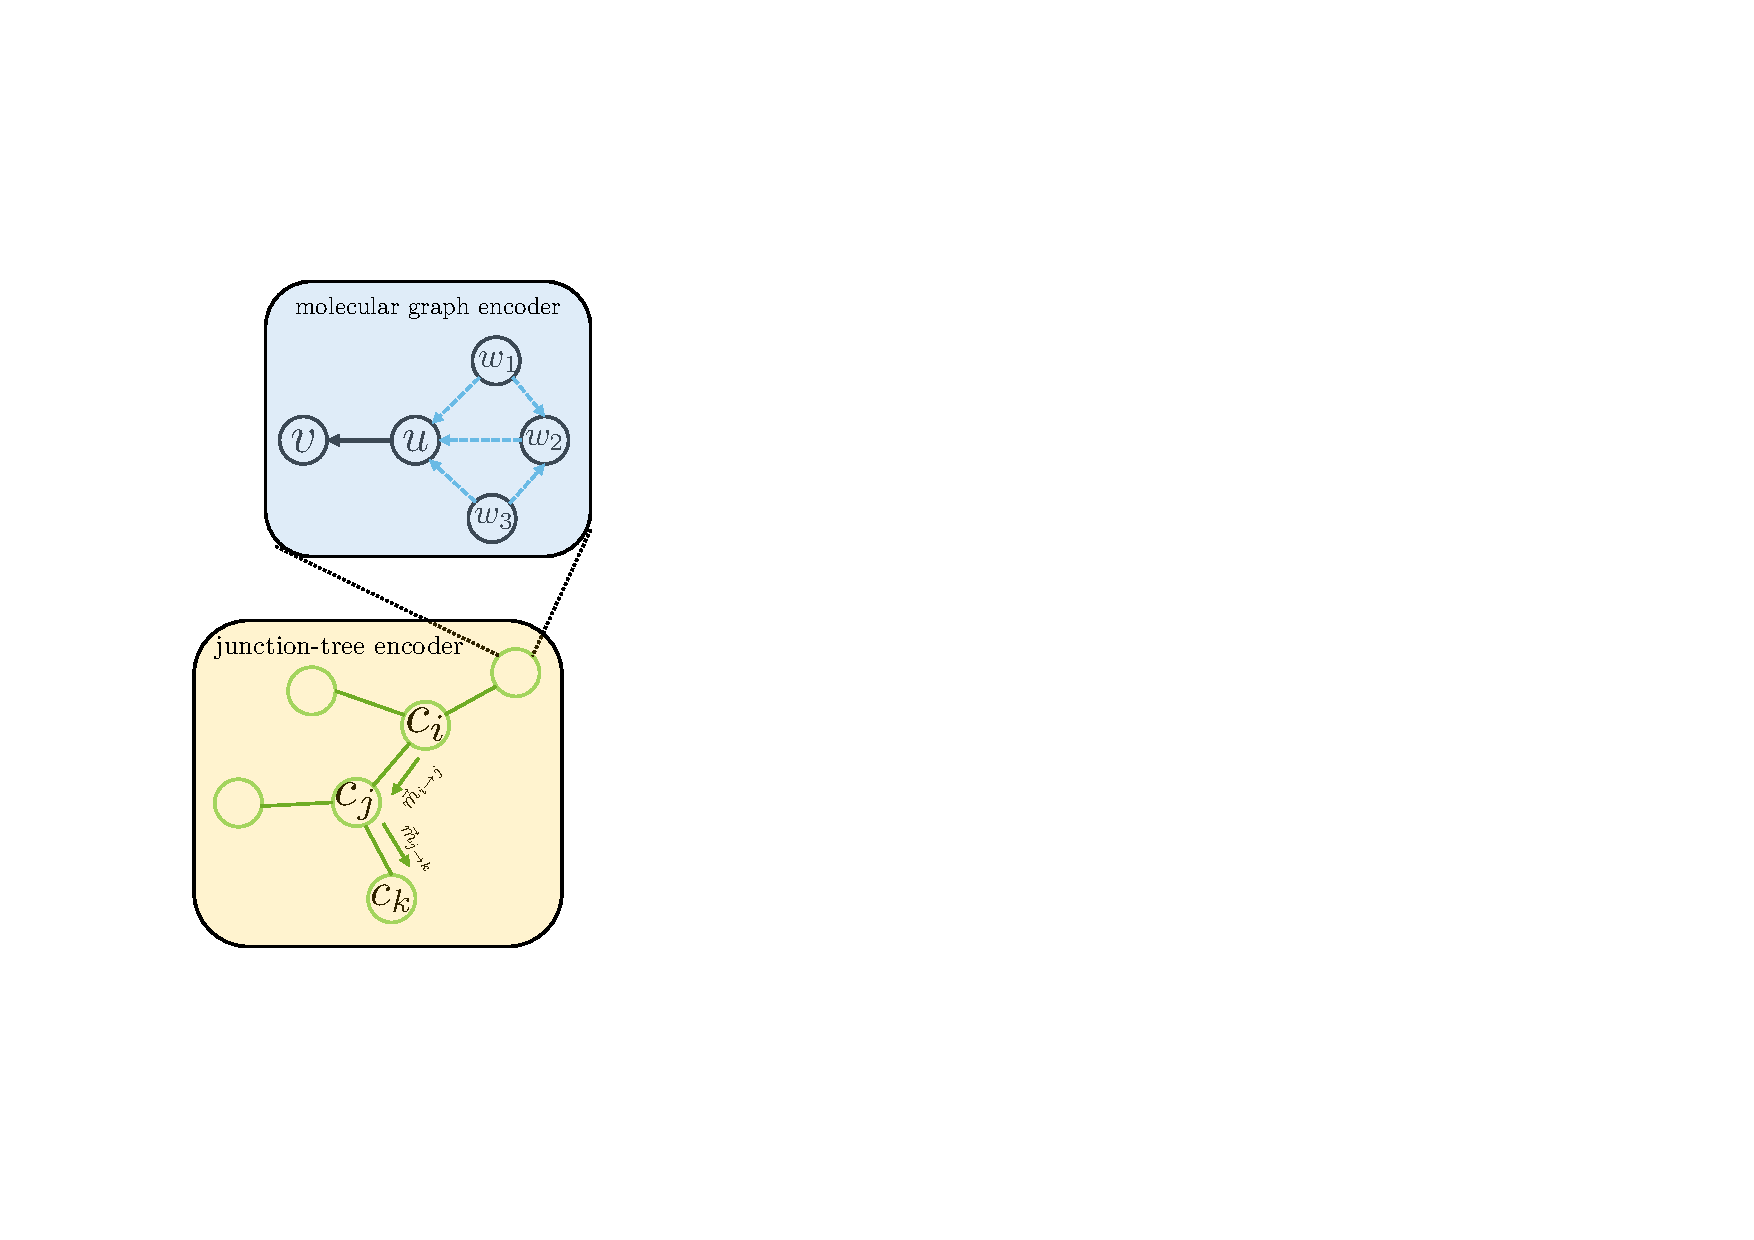
\includegraphics[width=0.3\textwidth]{junction-tree-net.pdf}
    \caption{Schematic illustrations on the hierarchical encoders in the junction-tree variational autoencoder\cite{jin2018junction} for molecular generation, in which a molecular graph encoder (blue box) is first deployed to encode (neighbouring) atoms into clusters, and a junction-tree encoder is then deployed to exchange information amongst clusters to build up the entire structure of the molecule.}
    \label{fig:junction-tree-net}
  \end{center}
\end{wrapfigure}
which is initialised with $\boldsymbol{\nu}_{wu}^{(0)}=0$. Essentially the last term in this operation progressively aggregates the information from all the neighbouring nodes $w$ (that are not $v$)  around $u$ to the central node $u$, before it is used to update the information encoding the bond that connects $u$ and $v$ (blue dashed arrows in the blue box of \cref{fig:junction-tree-net}). After $T$ MP operations, the message on a given node $u$ from all of its incoming bonds are aggregated into the final \emph{per-atom} representation:
\begin{equation*}
    \bm{h}_u=\tau\left( u_1^g\bm{x}_u + u_2^g\sum_{v\in\mathcal{N}(u)} \boldsymbol{\nu}^{(T)}_{vu}\right),
\end{equation*}
from which the global latent representation for the entire molecular graph $\mathcal{G}$ is averaged over all per-atom representations:
\begin{equation*}
    \bm{z}_{\mathcal{G}}=\frac{1}{\Vert V\Vert}\sum_{u\in V}\bm{h}_{u}.
\end{equation*}
This is similar to the construction of an averaged structural similarity kernel from atom-centred structural descriptors,\cite{de2016comparing} which was described in \cref{sec:physics_informed_representation}. The advantage of constructing the global latent representation of molecular structures is that in ensure molecules with different number of atoms are mapped into a latent representations with fixed dimensionality. However, it has essentially discarded the ordering information behind atomic connectivities, which makes it difficult to regenerate molecules based on $\bm{Z}_{\mathcal{G}}$ alone. It should be also easy to envisage that the way messages $\boldsymbol{\nu}^{(T)}_{vu}$ are aggregated does not depends on the topology of the molecular graph, so it should automatically be able to handle atoms that are interconnected in closed loop structures after some number of steps of MP.

\textbf{(ii) Junction-tree encoder through cluster-level message-passing}

\hspace{10pt} Here, the model treats the molecule as  clusters of atoms forming a tree-like graph structure without loop, which initiate itself from a single root that is sequentially branched into various leaves. (Whether all molecules confine with this directional tree-like structure, however, is questionable.) In this sense, the MP architecture should respect this directional tree-like structure.  

\hspace{10pt} To implement the junction-tree MP, we start from two interconnected clusters $\mathcal{C}_{i}$ and $\mathcal{C}_j$ in the junction tree $\mathcal{T}$ (yellow box of \cref{fig:junction-tree-net}), and we construct a \emph{directed message} $\bm{m}_{i\to j}$ that is computed from the label of cluster $\mathcal{C}_i$ and all messages entering $i$ from all of its neighbouring clusters other than $\mathcal{C}_j$:
\begin{equation*}
    \bm{m}_{i\to j}=\tau_{\mathrm{tree}}\left(\bm{x}_{i},\Big\{ \bm{m}_{k\to i} \Big\}_{k\in\mathcal{N}(i)\backslash j} \right).
\end{equation*}

\hspace{10pt} Here, the directional information is preserved by not explicitly aggregating the messages from all messages coming from nodes $\mathcal{C}_{k}$ into node $\mathcal{C}_j$ \textit{before} it is passed into $\tau_{\mathrm{tree}}$. More explicitly,   $\tau_{\mathrm{tree}}$ implements the following operations of MP:
\begin{enumerate}
    \item $\bm{s}_{ij}=\sum_{k\in\mathcal{N}(i)\backslash j} \bm{m}_{k\to i}$, which aggregate all messages coming into $\mathcal{C}_i$ from all neighbouring clusters $\mathcal{C}_k$ except $\mathcal{C}_j$.
    \item $\bm{z}_{ij}=\sigma\left(w^{z} \bm{x}_i+u^z \bm{s}_{ij}+\bm{b}^{z}\right)$, which is a gate operation that update the bonding information between  $\mathcal{C}_i$ and $\mathcal{C}_j$ based on the information on cluster $\mathcal{C}_i$  and $\bm{s}_{ij}$, the incoming information on $\mathcal{C}_i$. This is a standard message construction operation, which essentially gathers the information on how much  previously pooled bonding information affects the next one.
    \item $\bm{r}_{ki}=\sigma\left(w^r \bm{x}_i + u^r \bm{m}_{k\to i} +\bm{b}^r \right)$ for all $k\in\mathcal{N}(i)\backslash j$, which is a separate gate that update the information coming from each connected branch $k\to i$.
    \item $\bm{\tilde{m}}_{ij}=\tanh\left(w\bm{x}_i+u\displaystyle{\sum_{k\in\mathcal{N}(i)\backslash j}} \bm{r}_{ki}\odot  \bm{m}_{k\to i}\right)$, which gives a candidate message in which the weighting factor $\bm{r}_{ki}$ informs how much a particular branch $k\to i$ should influence the new message, and finally,
    \item $\bm{m}_{i\to j}=(\mathds{1}-\bm{z}_{ij})\odot \bm{s}_{ij}+\bm{z}_{ij}\odot\bm{\tilde{m}}_{ij}$.
\end{enumerate}
Similar to the all-atom MP operations outlined in (i), the junction-tree MP leas to the following per-cluster latent representation by gathering all the incoming messages to a specific cluster $\mathcal{C}_i$ as:
\begin{equation*}
    \bm{h}_i=\sigma \left(w^{o}\bm{x}_i+ \sum_{k\in\mathcal{N}(i)} u^{o} \bm{m}_{k\to i} \right),
\end{equation*}
and one simply takes the learned representation of the root node $z_{\mathcal{T}}=\bm{h}_0$ as the latent representation of the tree. More specifically, the junction-tree encoder implemented the MP operations along two directions. For MP from the root to the leaves, it will allow the leaves to receive instruction on whether to further branch out, whereas the information passed from the leaves to the tree enables the root to keep track on the global structures of the newly generated molecules. These are more specifically discussed as follows.

\textbf{(iii) Tree decoder that grows tree through message-passing}

\hspace{10pt} Taking the analogy from the MP operations in the tree encoding step, in the generative process, the model should decide whether one should generate a new node $\mathcal{C}_j$ from the current one $\mathcal{C}_i$ based on: (a) the features on $\mathcal{C}_i$, and (b) all other nodes $\mathcal{C}_k$ that had been traversed that lead to $\mathcal{C}_i$. Casting this mathematically, it reads
\begin{equation*}
    \bm{h}_{i\to j}=\tau_{\mathrm{tree}}\left(\bm{x}_i,\Big\{ \bm{h}_{k\to i}\Big\}\mbox{ for }(k,i)\mbox{ that has been traversed with } k\neq j\right).
\end{equation*}
 Practically, this message constructed is used by the decoder, upon reaching the tree node $\mathcal{C}_i$, to make a topological decision on whether to make a new node, or to backtrack:
\begin{equation*}
    p_j =\sigma\left( u^d\cdot \tau\left( w_1^d \bm{x}_i+w_2^d \bm{z}_{\mathcal{T}} +w_3^d \sum_k \bm{h}_{k\to i} \right) \right),
\end{equation*}
in which $\bm{z}_T$ is a new latent variable that is sampled in the sub-latent space for the junction-tree representations of molecule, this ensures that the generation process follows the conditional distribution $p(\mathcal{T}|\bm{z}_\mathcal{T})$ for the decoder. If a new leaf node $\mathcal{C}_j$ is created, then we can predict the actual cluster label for $\mathcal{C}_j$, which tells us what functional group should go into this particular cluster. Again, this will be conditioned upon $\bm{z}_T$  as:
\begin{equation*}
    q_{j}=\mbox{Softmax}\left(u^{l}\tau\left(w_1^l \bm{z}_{\mathcal{T}}+w_2^l \bm{h}_{i\to j} \right)\right).
\end{equation*}

\textbf{(iv) Graph decoder using tree-conditioned message-passing to assemble clusters}

\hspace{10pt} At this stage, all necessary components to build a new molecules would have been generated, and one is left with the final problem of identifying which pairs of atoms should be connected in order to join all the clusters together to form the final atomistic structure of the molecule. This is the reason why we need another full-atom MP scheme to update the bonding information. Following the notations used in the molecular graph encoder, we need a MP operation to update the bond connectivity between a candidate pair of atoms $(u,v)$, each coming from a different cluster that is connected between each other, mathematically, this reads
\begin{equation*}
    \boldsymbol{\mu}_{u\to v}^{(t)}= \tau\left(w_1^{\alpha} \bm{x}_u+ w_2^\alpha \bm{x}_{uv}+ w_3^\alpha \tilde{\boldsymbol{\mu}}_{u\to v}^{(t-1)}\right),
\end{equation*}
in which 
\begin{equation*}
    \tilde{\boldsymbol{\mu}}_{u\to v}^{(t-1)}=\sum_{w\in\mathcal{N}(u)\backslash v}\boldsymbol{\mu}_{u\to v}^{(t-1)}+\mathds{1}[\alpha_u\neq\alpha_v]\hat{\bm{m}}_{\alpha_u\to\alpha_v}.
\end{equation*}
Here, $\alpha_u$ bears the information on which cluster atom $u$ comes from, such that $\mathds{1}[\alpha_u\neq\alpha_v]\hat{\bm{m}}_{\alpha_u\to\alpha_v}$ can be considered as a penalty term that enforcing two interconnecting atoms must each comes from a different cluster. One may see that a potential bottleneck in this approach is that one must compute the message for all possible pairs of $(\alpha_u,\alpha_v)$ to optimise the connectivity of the fragments. 

\hspace{10 pt} Finally, one needs to assess the quality of the structure that is being generated by the model, which the authors proposed the score $f(\bm{G}_i)=\bm{h}_{G_i}^\top \bm{z}_{G}$ that measures the 
the alignment between the latent space representation $\bm{z}_{G}$ that is being sampled and the latent space representation (mapped by the all-atom encoder) for the molecules generated from the decoders. 
\end{myquote}


As one can see in the above discussions, a key aspect behind the designs of JTVAE for molecular structure generation is to progressively build the molecular framework (the tree) in a cluster-by-cluster manner. This progressive approach is similarly applied in the VAE model developed by  \citet{liu2018constrained} for molecular generation, in which, instead of trying to map a single $\bm{z}$ into a full atomistic molecular structure with the decoder, the model was designed to generate molecule atom-by-atom. At each generative step, the model first selects an atom of `current focus', and then decide whether one should add a new bond and atom, or the generative step should stop (through encountering a STOP signal). Practically, the generative model is designed to output a score $s_{vu}$ that can be used for determining the likelihood to generate a new bond between nodes $u$ and $v$, which is normalised amongst all possible nodes $\{u\}$ that might from a bond with $v$ as $p_{vu}=M_{vu}\exp(s_{vu})/\sum_w M_{vw}\exp(s_{vw})$, in which $M_{vw}$ allows to further implement a hard constraint for bond formation by defining $M_{vu}=1$ if a connection between $u$ and $v$ is allowed or zero otherwise. 

One of the key advantages to generate structures is the enabling of more fine-grained control on molecular structure generations, which leads to higher chance of generating valid structures. However, it is at the sacrifice on increasing model complexity, as can be seen from the discussions above. Nevertheless, one-shot approach to predict the global structures of molecules does exist, For example, in the same year as the VAE model proposed by \citet{liu2018constrained}, \citet{simonovsky2018graphvae} published the graph-VAE model for small molecular graph generation, which treats the entire molecular structure as a single graph $\mathcal{G}$, such that the VAE was designed to learn both the forward and backward conditional probability distributions between a graph and its corresponding latent space representations $p_{\boldsymbol{\theta}}(\mathcal{G}|\bm{z})$ and $q_{\boldsymbol{\varphi}}(\bm{z}|\mathcal{G})$. On a more practical level, the problem of structure generation become further simplified into the problems of predicting the adjacent matrix $\tilde{\bm{A}}\in[0,1]^{k\times k}$ for a molecule containing $k$ atoms, which defines the atomic connectivities. 

As a last, and more recent example of (progressive) molecule generations with the VAE framework, we examine the NEVAE model put forward by \citet{samanta2020nevae} Similar to the JTVAE model, rather than mapping an entire molecule $\{\bm{C},\bm{R}\}$ (chemical identity and atomic position vectors) into a single laten variable $\bm{z}$, NEVAE tries to map each atom in a molecule into a separate latent space variable as $\bm{z}=\{\bm{z}_1,\bm{z}_2,\cdots, \bm{z}_n\}$. The encoder then takes the inspirations from MPGNN that aggregates information up to $k$-th connected atoms in distant into the message $\bm{h}_i$. More specifically, the model implements this aggregation operation to be a symmetric one, such that the aggregated information does not depend on the order of atomic connectivities. This can be achieved with, for example, a summation operation as
\begin{equation*}
    \begin{cases}
        \phi(\bm{h}_i) \to\bm{z}_i\\
        \bm{h}_{i}^{(k)}=f_k\left( \bm{h}_i^{(k-1)},\mbox{AGG}\left\{  g_k\left(\bm{h}_j^{(k-1)},\bm{e}_{ij}\right): j\in \mathcal{N}(i)\right\} \right).
    \end{cases}
\end{equation*}
Similarly, the decoder in the VAE generates molecular structures in stages. Here, starting from the number of atoms $n\sim\mbox{Poisson}(\lambda_n)$, the model first sample the per-atom latent variables $\bm{z}_i\sim\mathcal{N}(0,\bm{I})$, from which the corresponding atom type is determined based on a learned conditional probability distribution of $p(x_i=C|\bm{z}_i)$. Subsequently, the latent variables $\bm{z}_i$ are used for sampling the number of bonds from $m\sim\mbox{Poisson}(\lambda_{E}(\bm{z}))$ such that the model knows how many edge-generation decisions it needs to make. From here, the model then builds an edge between any two nodes $i$ and $j$ based on a computed probability for edge formation that is similar to \citet{liu2018constrained}. The model then determines the bond type for each connection and finishes by sampling the 3D coordinates for each atom. 

\paragraph{\textbf{Generation of Crystalline Solids}}
Moving on to the designs and implementations of VAE-based generative models for crystalline materials. The model put forward by \citet{noh2019inverse} was one of the earliest proof-of-concept generative models for  inorganic crystals, which had already demonstrated performances that were comparable to traditional genetic algorithms. As mentioned by the authors, the key advantage in VAE-based crystal structure prediction compared to genetic algorithm is that the former is physically grounded by the probability distributions of the \emph{thermodynamically stable} crystal structures, which should naturally enhance the successful rates in generating feasible inorganic crystal structure. Being a model that was developed pre-dating the uprise of equivariant NNs, the model drew analogy of structure generation to that of image generations by mapping the positions of atoms inside a cubic box into an atom-centred Gaussian distributions inside a pixelated 3D grid, which is learnt by the model and also acts as the target generative outcome for the backward decoder.

\citet{xie2021crystal} proposed the crystal diffusion variational autoencoder (CDVAE) that combined the frameworks of VAE and diffusion models for generating periodic crystal structures. Here, the encoder of the VAE tries to learn a parameterised conditional distribution $q_{\boldsymbol{\phi}}(\bm{z}|\bm{M})$ of the latent representation $\bm{z}$ for a given crystal structure $\bm{M}$ that is collectively represented by $(\bm{A},\bm{X},\bm{L})$, which denotes the atomic number, atomic coordinates, and the lattice parameters of the crystal, respectively. To generate a new sample of the crystal structure, one first samples a new variable $\bm{z}^\prime$ in the latent space, which is then put into the decoder to generate a \emph{coarse} initial structure of $\tilde{\bm{M}}_0=(\tilde{\bm{A}}_0,\tilde{\bm{X}}_0,\hat{\bm{L}})$. Then the mode uses the score function to progressively refine the chemical identity and the atomic positions with a diffusion model: $(\tilde{\bm{A}}_0,\tilde{\bm{X}}_0)\to\cdots\to(\tilde{\bm{A}}_\mathrm{final},\tilde{\bm{X}}_\mathrm{final})$. Note that, if we do not wish to refine the chemical identities, but only the positions of the atoms in the crystal that is being generated, the score function essentially resembles an atom-atom forcefield (as discussed in \cref{sec:common_generative_models}), meaning that the refining step is equivalent to the use of an energy function to optimise the newly generated structure to a nearby local energy minimum. In this sense, this particular VAE framework can be conceptually understood as a simulated annealing process that first samples a structure on a high-temperature PES to overcome the problem of crossing high energy barriers in traditional MD/MC-based approaches [\cref{sect:MonteCarlo} and \cref{sect:molecular_dynamics}], followed by quenching the structure into a stable one. To provide an example of property-guided structure generation, \citet{luo2024deep} extended the CDVAE\cite{xie2021crystal} model for generating high-pressure crystal structures, which is achieved by further augmenting the vectorial representation of crystal structure with an additional term that encodes the information of pressure $P$. The later was realised by mapping $P$ onto a basis constructed using equidistant Gaussian functions.

The Wyckoff positions for atoms  are unique symmetry-embedded encoding of atomic positions in a crystal structure, for this reason, the WyCryst model proposed by \citet{zhu2024wycryst} explored the usage of the  Wyckoff positions for representing and generating candidate inorganic crystal structure. Different from the CDVAE model, WyCryst seeks to represent a given crystal structure as a tuple of $\bm{W}_i=(\bm{X}_i,\bm{S}_i,\bm{F}_i)$, which correspond to the Wyckoff positions, one-hot-encoded space group and chemical element representations, respectively. This allows the VAE model developed to learn the statistical distribution (as a function of $\bm{W}$) for all inorganic crystals in the training data. One could identify multiple advantages in using the Wyckoff representations for the tasks of inorganic crystal structures. For examples, the Wyckoff positions naturally define a constrained space $\bm{X}_i\in[0,1)^3$ that is beneficial for enhancing the learning and inference stabilities of the model. Utilising the Wyckoff positions also reduces the dimensionality of the problems to be tackled, as one only needs to generate atoms in a set of unique symmetry-inequivalent Wyckoff sites, and complete the whole crystal by using the symmetry operations (which is also called the \emph{generators} that are embedded in $\bm{S}_i$) to generate the other symmetry-related Wyckoff positions. This also overcomes the problem of permutation invariance in structure generations, when only a single site amongst a set of symmetry-related Wyckoff positions is needed for model learning and inference. The complexity of the problem can be further reduced  by realising the fact that many special Wyckoff positions are fixed (such as $(0,0,0)$ and $(\frac{1}{2},\frac{1}{2},\frac{1}{2})$), or contain fewer independent parameters (such as $(x,\frac{1}{4},\frac{1}{4})$ with $x\in[0,1)$). A possible extension of Wyckoff-position-based generative models for inorganic crystal could be through the explorations of packing different `packing-motifs' (such as octahedra and tetrahedra), that are represented by a group of related Wyckoff positions, to develop crystal generative models with greater physical and structural interpretability. 

Finally, to highlight the cross-disciplinary nature in the development of AI for scientific discovery, we discuss the model developed by \citet{chen2025transformer} which utilised the transformer architecture\cite{vaswani2017attention} from the large language model for the task of crystal structure prediction. Here, instead of using GNN, the transformer is applied to encode the latent representation $\bm{z}$ for a given crystal structure. This is inspired by the fact that, the distributions of the neighbouring coordination environments in an inorganic crystal structure are highly correlated thus non-uniform, in which certain pairs of neighbouring atoms (\emph{e.g.} a cation surrounded by anions) are more likely to occur compared to the other pairs, which is highly similar to the appearance of word sequences in sentences. Here, each local environment around a given centre is first encoded into a set of SO(3) equivariant features up to a prescribed order $n$ as $\bm{h}_i=[\bm{h}_i^{(0)},\bm{h}_i^{(1)},\cdots,\bm{h}_i^{(n)}]$. Then the transformer learns the attention coefficient $\alpha_{ij}\propto \bm{h}_i\cdot\bm{h}_j$ amongst all pairs of chemical environments, which provides the information on the likelihood that a pair of atomic environments may occur as neighbour to each other. Most importantly, the structural equivariance (and hence the equivariance in the attention coefficient thus computed) can be strictly imposed if the attention coefficients are computed by following the group representation theory (see \cref{sec:physics_informed_representation}). Furthermore, the model developed a dataset-adaptive encoding scheme for better encoding the interatomic distances $r_{ij}$  into their respective latent space representation, for example, the authors had chosen to map $r_{ij}$ for the \texttt{MP-20} training set into equidistant Gaussians, whereas for the \texttt{Perov-5} set (which are structurally more uniform), $r_{ij}$ is mapped into a set of Bessel functions, which are itself oscillatory in nature that better reflects the periodicity of the crystal structures. 

\subsubsection{Applications of Diffusion Generative Models in Atomistic Modelling}
\label{sec:generative_diffusion_examples}


Since around 2020, diffusion generative model\cite{ho2020denoising} has become one of the dominant and rapidly-developing deep generative model, particularly for its demonstrated capability to generate images with higher qualities compared to the GAN (Generative Adversarial Network) model.\cite{dhariwal2021diffusion} In the field of atomistic molecule and material generations, the development of diffusion model has been a vibrant multidisciplinary field in model development, requiring the practitioners in this particular area to possess a wide range of knowledges to further advance the field. These include: (a) Probability theory, particularly in terms of the Bayesian statistics [\cref{sec:prob_theory_fundamentals}], which plays an important role in determining the appropriate probability distributions that the system should follow, such that the forward and reverse diffusion processes are implemented in a way that these distributions are respected. (b) Choosing the appropriate way to represent the atomistic structures as the learning and generative targets. (c) Fundamentals of group and representation theories [\cref{sec:physics_informed_representation}] that enables the NN models to learn the noises while respecting the invariant and equivariant symmetries of the systems to be modelled. (d) Stochastic processes, that is grounded by the SDE formulation of the diffusion model [\cref{eq:diffusion_forward_SDE} and \cref{eq:reverse_generation_SDE}] which enables one to explore \cite{song2020score,song2020denoising} the mathematical techniques in solving differential equations to accelerate the sampling of new materials, as well as designing a diverse range of data-dependent forward collapsing process of the input data.\cite{cornet2024equivariant} (e) Differential geometry, which enables one to design the coordinate-specific transformation of atomistic structures on the high-dimensional manifold, and derive the corresponding score functions for model training. Finally, (f) Statistical mechanics, which provides the conceptual bridge to derive the physical interpretation of the SDE with the conventional energy-based PES samplings [\cref{chapter:sampling_methods}].

In this regard, the development of diffusion generative models is largely the process of exploring and incorporating different mathematical techniques that have been developed for the subfields listed above, to improve the model efficiency, stability and capabilities to extrapolate beyond the known materials space. These requirements may be much beyond the knowledge base for general materials modellers, which poses a significant challenges for them to develop deep understanding on the key features in the models that have been developed and why they may be applicable to specific categories of targeted materials systems. Hence, the purpose of this section is aiming at providing the community with an overview on how the above listed aspects are intertwined together in the designs and implementations of diffusive generative models for molecules and crystalline materials through a chronological review of the diffusion generative models proposed over the recent years. In particular, we aim to highlight how the model design are strongly influenced by the design choices on how the structure and chemistry are represented as the training and generative targets for the diffusive generative models.

\paragraph{\textbf{Generation of Molecules}}
 Following the same sequence as the discussions around VAE models, we begin here by reviewing different implementations of the diffusion generative models that have been developed for the task of molecular structure generations. \citet{niu2020permutation} presented one of the earliest diffusion models for generating graph objects, that is applicable for molecules when being treated as graphs, in which the molecular generation task is being cast here as one that samples different adjacency matrices $\bm{A}$ for representing the molecular graphs with the diffusion generative model. In this regard, a key considerate when constructing the NN model to approximate the score function $s_{\boldsymbol{\theta}}(\bm{A})=\nabla_{\bm{A}}\log p_{\boldsymbol{\theta}}(\bm{A})$ is the \emph{permutation invariance of graph} (also \emph{c.f.} \citet{simonovsky2018graphvae}), meaning that with $\Pi$ being the set of row/column permutation operations on $\bm{A}$, then: (a) $\forall \pi_i,\pi_j\in\Pi$ and $\pi_i\neq\pi_j$, $s_{\boldsymbol{\theta}}(\pi_1(\bm{A}))=s_{\boldsymbol{\theta}}(\pi_2(\bm{A}))$, which can be achieved with NN operations that only operates element- or edge-wise, or not sensitive to the atomic ordering, such as the aggregation operations, as well as explicitly constructing the score function to be symmetric thus permutation invariant \emph{e.g.} $s=\left(s+s^\top\right)/2$. Furthermore, the author pointed out an important geometric interpretation of the score function $s(\pi(\bm{A}))$, which is the gradient along a specific transformation pathway from a noised starting point $\bm{A}=\bm{0}$ to $\pi(\bm{A})$,  hence the final log-probability distributions over graphs $\log p(\bm{A})$ can be obtained by integrating $\langle s(\bm{X}),d\bm{X}\rangle_F$ (with $\langle\cdot\rangle_F$ being the  Frobenius inner product)  over all possible transformation pathways in the diffusion process. Conceptually, this resembles the construct of \emph{averaged} structural similarity kernel\cite{de2016comparing} in atomistic machine learning (\cref{sec:feature_eng}) that removes the problem of permutational matching of atom pairs. In this case, with the NN-modelled score function $s_{\boldsymbol{\theta}}(\bm{A})$ being permutational invariant will also ensure $p(\bm{A})$ is also permutational invariant.  (b) One must also ensure that in the reverse diffusion process that samples the adjacent matrix does not repetitively samples adjacent matrices that are the permuted copies of each other. For this, the author proposed that with learnt $s_{\boldsymbol{\theta}}(\bm{A})$, the sampling process can start with $\tilde{\bm{A}}^{(T)}$ with $\tilde{\bm{A}}_{ij}^{(T)}\sim\mathcal{N}(0,1)$ and $\tilde{\bm{A}}_{ij}^{(T)}=\tilde{\bm{A}}_{ji}$, followed by repretitive sampling using Langevin dynamic as $\tilde{\bm{A}}_{ij}^{(t-1)}=\tilde{\bm{A}}_{ij}^{(t)}+\frac{\alpha_t}{2}s_{\boldsymbol{\theta}}(\tilde{\bm{A}}^{(t)},\sigma_t)+\sqrt{\alpha_t}\bm{Z}_t$, whereby $\bm{Z}_t$ is a symmetric Gaussian noise that is added to prevent the sampling from converging prematurely to regions with high probability. Readers may already appreciate from this early work that, even though the underlying object being transformed (the adjacency matrix $\bm{A}$ with $\bm{A}_{ij}\in[0,1]$) may be quite simple, the  details to be considered in designing mathematical transformations of this object through diffusion model while ensuring permutational invariance is already very involved.

To progress one step further from a binary encoding of atomic connectivities, \citet{shi2021learning} addressed the problem of generating the 3D coordinates $\bm{R}$ for molecules from a given molecular graph $\mathcal{G}$ via the interatomic distances, in which case the model needs to learn a score function with respect to $\bm{R}$ that is conditioned on $\mathcal{G}$, \emph{i.e.} $s_{\boldsymbol{\theta}}(\bm{R}|\mathcal{G})=\nabla_{\bm{R}}p(\bm{R}|\mathcal{G})$. In particular, this model utilise the chain rule to reach an explicit expression of the score function with respect to the atomic coordinates and interatomic distances as $s_{\boldsymbol{\theta}}(\bm{R}_i)=\sum_{j\in\mathcal{N}(i)}s_{\boldsymbol{\theta}}(d_{ij})(\bm{R}_i-\bm{R}_j)/d_{ij}$, which is a quantity that is rotational and translational invariant up to 2-body, and can be learnt with GNN models that implement invariant operations at this body-order (\cref{tab:equivariant_GNNS}). With this learnt score function, the model can then achieve the sampling of atomic positions, starting from a random geometry, and progressively denoised following the Langevin dynamics.

\citet{jo2022score} further consider the molecular representation as a full graph $\mathcal{G}=(\bm{X},\bm{A})$ in which $\bm{X}\in\mathbb{R}^{N\times F}$ is the node feature vector for $N$ nodes each with a dimension of $F$, and $\bm{A}\in \mathbb{R}^{N\times N}$ is the \emph{weighted} adjacency matrix. The main uniqueness behind this work, is that, rather than simply just adding the Gaussian noise to collapse the samples, it evolves $\bm{X}$ and $\bm{A}$ separately in the forward process by designing the according SDEs [\emph{c.f.} \cref{eq:diffusion_forward_SDE}]:
\begin{equation}
    \label{eq:JLH_forward_SDE}
    \begin{cases}
        \mathrm{d}\bm{X}_t=f_{1,t}(\bm{X}_t)dt+g_{1,t}\mathrm{d}\bm{w}_{1,t}\\
        \mathrm{d}\bm{A}_t=f_{2,t}(\bm{A}_t)dt+g_{2,t}\mathrm{d}\bm{w}_{2,t},
    \end{cases}
\end{equation}
in  which $\mathrm{d}\bm{w}\in\mathcal{N}(0,\bm{I})$. Hence this generative model extended the previous two by allowing both the chemistry and the structure of the molecule to be changed in the diffusion process. The main advantage of using SDEs for the forward process is that it can better ensure the finally collapsed samples are well centred around a predefined mean (typically zero), such that the original sample can be gradually collapsed by following a noise with well defined variance to ease the subsequent samplings. This may be achieved, for example, by designing the appropriate drift functions $f$ for different parts of molecular representations. Following \cref{eq:JLH_forward_SDE}, the model needs to train two score functions 
\begin{equation*}
    \begin{cases}
        s_{\boldsymbol{\theta},t}(\bm{X}_t,\bm{A}_t) = \nabla_{\bm{X}_t}\log p_t(\bm{X}_t,\bm{A}_t)\\
         s_{\boldsymbol{\varphi},t}(\bm{X}_t,\bm{A}_t) = \nabla_{\bm{A}_t}\log p_t(\bm{X}_t,\bm{A}_t)
    \end{cases}
\end{equation*}
that are to be used in the generating process with the reverse SDE [\emph{c.f.} \cref{eq:reverse_generation_SDE}]:
\begin{equation*}
    \begin{cases}
        \mathrm{d}\bm{X}_t = \left[f_{1,t}(\bm{X}_t)-g_{1,t}^2s_{\boldsymbol{\theta},t}(\bm{X}_t,\bm{A}_t)\right]\mathrm{d}t +g_{1,t}\mathrm{d}\bm{w}_{1,t}\\
        \mathrm{d}\bm{A}_t = \left[f_{2,t}(\bm{A}_t)-g_{2,t}^2s_{\boldsymbol{\varphi},t}(\bm{X}_t,\bm{A}_t)\right]\mathrm{d}t +g_{2,t}\mathrm{d}\bm{w}_{1,t}.
    \end{cases}
\end{equation*}
Since both score functions are modelled as the joint probability distribution that is dependent on the adjacency matrix $\bm{A}$, one can appreciate that the above discussion on implementing NN approximator that preserves the \emph{permutation invariance} is also a necessary model design constraint here.

\citet{wu2022diffusion} also harnessed the flexibility of SDE in the design of diffusion generative model, which they considered the drift-term $f(\bm{x})\sim p_t(\bm{x}_t|\bm{x}_0)$ as determined by a time-dependent probability distribution that is conditioned upon the training samples $\bm{x}_0$. This enables them to design the drift term by including an additional \emph{informative bias force} that is force-field based to evolve samples into physically and statistically meaningful distribution, $\emph{i.e.}$
\begin{equation*}
    p_t(\bm{x}_t|\bm{x}_0)=\underbrace{\sigma_t^2\frac{\bm{x}_0-\bm{x}_t}{\beta_t-\beta_0}}_{\mbox{\scriptsize{Brownian term}}}+\underbrace{\sigma_t\left(-\nabla_{\bm{x}_t}E(\bm{x}_t)\right)}_{\mbox{\scriptsize{Informative bias force}}}.
\end{equation*}
As demonstrated in the paper, a possible choice of $E(\bm{x})$ is the traditional atom-atom forcefield [\emph{c.f} \cref{sect:empirical_forcefield}], but this does not exclude the use of modern NN forcefields [\cref{tab:equivariant_GNNS}] in which \emph{per-atom} gradients are available. The model training process then adopt the score-matching process, in which the conditional distribution $p_t(\bm{x}_t|\bm{x}_0)$ becomes the learning target for the score function. 

\citet{xu2022geodiff} designed the \textsc{GeoDiff} model for molecular conformation generation. Conceptually, the authors treat both the forward and backward diffusion processes as the Markov chains with the corresponding transition probabilities $q(\bm{x}_{t}|\bm{x}_{t-1})$ and $p(\bm{x}_{t-1}|\bm{x}_t)$ being treated as the Markov transition kernels. Based on this formulation, the model focuses on designing transition kernels that are SE(3)-equivariant, meaning that  $\forall\hat{\mathcal{T}}_g\in$SE(3), it follows $p(\bm{x}_{t-1}|\bm{x}_t)=p\left(\hat{\mathcal{T}}_g\left(\bm{x}_{t-1}\right)|\hat{\mathcal{T}}_g\left(\bm{x}_t\right)\right)$. This is achieved by designing the kernel as 
\begin{equation*}
    \hat{\rho}\left(\frac{\bm{x}_{t-1}-\mu_{\boldsymbol{\theta}}(\mathcal{G},\bm{x}_t,t)}{\sigma_t}\right),
\end{equation*}
which is naturally conditioned on a given molecular graph $\mathcal{G}$, with the molecular conformations $\bm{x}_{t}$ and $\bm{x}_{t-1}$ centred around their respective centres-of-masses to remove the translational degree-of-freedom, while the rotational equivariance is further imposed by using an equivariant Graph Field Network\cite{satorras2021n} to parameterise the mean as 
\begin{equation*}
    \mu_{\boldsymbol{\theta}}(\mathcal{G},\bm{x}_t,t)=\frac{1}{\alpha_t}\left(\bm{x}_t -\frac{\beta_t}{\sqrt{1-\bar{\alpha}_t}}\varepsilon_{\boldsymbol{\theta}}(\mathcal{G},\bm{x}_t,t) \right).
\end{equation*}
Up to this stage, the model still resemble a standard diffusion generative model. The main innovation of this work lies in how the authors formulated the model training processes. In the first variant, the model derived the training loss following the minimisation of ELBO which essentially cast the training process into the minimisation of $\left\Vert \boldsymbol{\varepsilon}_t -\varepsilon_{\boldsymbol{\theta}}(\bm{x}_t,t) \right\Vert_2^2$, in which $\boldsymbol{\varepsilon}_t\sim \frac{1}{\sqrt{1-\bar{\alpha}_t}}\left(\bm{x}_t-\sqrt{\bar{\alpha}_t}\bm{x}_0\right)$ that are computed by taking the differences of two molecular conformations. The model solve this problem by first overlaying the centres-of-masses between the two conformations followed by the solution of the optimum rotational matrix using the Kabsch algorithm to align them before the differences are taken. This nonetheless introduces additional computational costs in each step of the reverse diffusion process, and may lead to the problem of the noise $\boldsymbol{\varepsilon}_t$ no longer following a white noise as the Kabsch algorithm may not always find the global minimum for the rotation matrix, leading to instabilities in the reverse generation process.  In the alternative variant to mitigate the alignment problem, the author followed the score-matching framework used by \citet{shi2021learning}, which allows the time-dependent noise to be computed based on the differences in pair-wise interatomic differences $\boldsymbol{\varepsilon}_t\sim\frac{1}{\sqrt{1-\bar{\alpha}_t}}[\partial_{\bm{x}_t}\bm{d}_t\cdot\left( \bm{d}_t-\sqrt{\bar{\alpha}_t}\bm{d}_0 \right)]$ that can be approximated with a two-body invariant GNN.
We note that this alignment problem is usually overcome in later model by learning and directly using $\boldsymbol{\varepsilon}_{\boldsymbol{\theta}}$ modelled by equivariant NN.

The model developed by \citet{hoogeboom2022equivariant} in 2022 is a landmark $E(3)$-equivariant model that jointly diffuse the atomic coordinates (continuous features) and atomic types (categorial features), building on the standard diffusion denoising probabilistic model (DDPM)\cite{ho2020denoising} and the Markov transition formalism by \citet{xu2022geodiff}. In particular, the model harness the two-body invariant EGNN model\cite{satorras2021n}, together with the inspirations of the score functions from \citet{shi2021learning}, to learn the noises that are dependent on both the coordinates $\bm{x}_i\in\mathbb{R}^3$ and nodal features $\bm{h}_i\in\mathbb{R}^d$ through the following the following message constructions:
\begin{equation}\label{eq:Hoogeboom_MP}
    \begin{cases}
        \bm{m}_{ij}=\phi_{e}\left(\bm{h}_i,\bm{h}_j,\bm{d}_{ij},a_{ij}\right),\\
        \bm{h}_{j}^{(\ell+1)}=\phi_{h}\left( \bm{h}_i^{(\ell)},\sum_{ij}\tilde{\bm{e}}_{ij}\bm{m}_{ij}\right),\\
        \displaystyle{\bm{x}_i^{(\ell+1)}=\bm{x}_i^{(t)}+\sum_{j\neq i}\frac{\bm{x}_i^{(\ell)}-\bm{x}_j^{(\ell)}}{d_{ij}+1}\phi_{x}\left(\bm{h}_i^{(\ell)},\bm{h}_j^{(\ell)},d^2_{ij},a_{ij}\right)}.
    \end{cases}
\end{equation}
In which $\ell$ is the index of the MP layer.
With this model, for each input structure $\bm{x}_t$, the model is able to directly learn the time-dependent noise $\boldsymbol{\varepsilon}_{\boldsymbol{\theta}}(\bm{x}_t,t)$ that is invariant with respect to  the ro-translations of $\bm{x}_t$. In addition, the intermediate diffusion steps jointly diffuse both the coordinates $\bm{x}_{t}$ and the feature $\bm{h}_{t}$ that samples both the molecular chemistry and structures together, for which the Markov transition probability\cite{xu2022geodiff} needs to be extended to reflect the joint probability distributions of the structure- and chemistry-dependent noises. By explicitly parameterising this joint distribution as $\mathcal{N}\left(\left .\bm{z}_t^{(\bm{x})}\right\vert \bar{\alpha}_t\bm{x}_0,\bar{\sigma}_t^2\bm{I}\right)\cdot \mathcal{N}\left(\left .\bm{z}_t^{(\bm{h})}\right\vert \bar{\alpha}_t\bm{h}_0,\bar{\sigma}_t^2\bm{I}\right)$, the model is trained to predict structure- and chemistry-dependent noises that can be concatenate together to assemble a total time-dependent noise $\boldsymbol{\varepsilon}_t=(\boldsymbol{\varepsilon}_t^{(\bm{x})},\boldsymbol{\varepsilon}_t^{(\bm{h})})^\top$. This allows one to sample molecular structure in the denoising process as $(\bm{x}_{t-1},\bm{h}_{t-1})^\top=\frac{1}{\alpha_t}[(\bm{x}_{t},\bm{h}_{t})^\top-\boldsymbol{\varepsilon}_t\sigma_t]$ with the initial state of $(\bm{x}_T,\bm{h}_T)$ drawn from their respective probability distributions that should be followed. Subsequently, \citet{igashov2024equivariant} extended this model for the conditional design of molecular linkers, whereas \citet{schneuing2024structure} further tailored the model for structure-based drug designs with equivariant diffusion.

Similarly, \citet{huang2023mdm}  adopted the SchNet\cite{schutt2017schnet} [\emph{c.f.} \cref{tab:equivariant_GNNS}] to enable the learning of equivariant score $s_{\boldsymbol{\theta}}(\bm{x}_t)$ that leads to a similar two-body form of the score function as \citet{shi2021learning} to achieve the generation of new molecular structure. An additional noise term is incorporated into the revserse sampling process to enhance the diversification of the samples being generated by the diffusion model


As discussed in \cref{sec:descriptor_motivation},  choosing the appropriate coordinates system plays an important role in determining the sampling efficiency. In this regard,  \citet{jing2022torsional}  considered the diffusion generative process for conformational flexible molecules in the space of torsional angle that operates on a hypertorus $\mathbb{T}^{m}$ of $m$ torsional angles. Correspondingly, the distribution of torsional angles $\boldsymbol{\tau}\in[0,2\pi)^m$ follow  that of a wrapped normal distribution that should be respected in the diffusion generative process (\emph{c.f.} \cref{tab:continuous_prob_distributions}), as they do not live in the usual Cartesian space of $\mathbb{R}^{m}$. In this case, the diffusion process on $\mathbb{T}^{m}$ can be efficiently implemented as $\boldsymbol{\tau}_{t+1}=\left(\alpha_t\boldsymbol{\tau}_t+\beta_t\boldsymbol{\varepsilon}_t\right)\mbox{mod 2}\pi$, with $\boldsymbol{\varepsilon}_t\sim\mathcal{N}(0,\bm{I})$, that properly ensures $\forall\boldsymbol{\tau}_t\in[0,2\pi)^m$.
However, the author also noted that the knowledge of a complete set of $\{\tau_i\}_{i=1}^{m}$  does not directly lead to a new molecular structure. To address this problem, the model adopted an extrinsic-to-intrinsic score model that first receives the current molecule as a 3D point cloud, then predict and assign a torsion angle for each rotatable bond. Physically, the as-proposed model can be considered equivalent to the establishment of a torsion-angle-dependent energy model for sampling the molecular conformation,\cite{cheng2024response} or a Boltzmann machine\cite{noe2019boltzmann} that draws samples of torsion angles from the distributions of which that are seen in the stable molecules.

\citet{vignac2022digress} developed the \textsc{DiGRESS} model, which can be considered as a diffusion-based editing model, that aims to generate graph objects $\mathcal{G}$ with edges and nodes that both follow discrete categorial distributions. This leads to the Markov transitions that  edits the graphs by successively adding or deleting nodes and edges, or mathematically expressed as $q(\bm{x}_{i,t}|\bm{x}_{i,t-1})=\mbox{Pr}_{x,t}(x=i)$ and $q(\bm{e}_{ij,t}|\bm{e}_{ij,t-1})=\mbox{Pr}_{E,t}(E=ij)$, which can be use to train a model $p_{\boldsymbol{\theta}}(\mathcal{G}_{t-1}|\mathcal{G}_t)$ through minimising a loss function based on cross-entropy $\mathcal{L}=\sum_i\mbox{CE}(\bm{x}_i,\hat{\bm{x}}_{i})+\sum_{ij}\mbox{CE}(\bm{e}_{ij},\hat{\bm{e}}_{ij})$. 
With the trained transition kernel, the reverse generation  process $\mathcal{G}_T\to\cdots\to\mathcal{G}_0$ can be proceeded by successively applying the graph editing operation. One can easily envisage that, similar to \citet{niu2020permutation}, enforcing the permutation invariance would be the key design constraint in designing the NN that learns the Markov transition kernels. Subsequently, the same group of authors\cite{vignac2023midi} further advanced the \textsc{DiGRESS} model that leads to the \textsc{MiDi} model for the task of molecular generation by simultaneously generating both the 2D connectivity and 3D structures, with the additional capabilities of generating the formal atomic charges. The model is designed based on representing the molecular graph as $\mathcal{G}=(\bm{X},\bm{C},\bm{R},\bm{Y})$, which correspond to the vectors representing the atom types, formal charges, and matrices representing the atomic coordinates and bond types, respectively. Hence, the probability distribution over the molecular graphs now follows a mixture of continuous and discrete distributions, which is reflected in the modified training loss $\mathcal{L}=\lambda_{\bm{R}}\Vert \hat{\bm{R}}-\bm{R}\Vert_2^2 +\lambda_{\bm{C}}\mbox{CE}(\hat{\bm{C}},\bm{C})+\lambda_{\bm{X}}\mbox{CE}(\hat{\bm{X}},\bm{X})+\lambda_{\bm{Y}}\mbox{CE}(\hat{\bm{Y}},\bm{Y})$, in which the part contributed from $\bm{R}$ follows that of the standard diffusion model on continuous variables whose distribution is parameterised as the normal distribution.\cite{ho2020denoising} Such design of the training loss naturally takes into account the interdependencies among the four variables that constitutes the full representation of $\mathcal{G}$, or equivalently, the 3D atomistic structures of the molecules. Implementation-wise, the model adapted a modified EGNN\cite{satorras2021n} for predicting the Markov transition probabilities, enforcing two-body equivariance in the model training and inference.
 
The MuDiff model proposed by \citet{hua2024mudiff} shares similar design concept as \textsc{MiDi} whereby the model also tries to generate both the 2D graph and the 3D molecular structures simultaneously, except they adopt a molecular representation in the form of $\mathcal{M}=(\bm{H},\bm{E},\bm{X})$, which correspond to the atomic features, edge features and the matrix of the Cartesian coordinates, respectively. Consequentially, this also leads to a loss function that is established based on a mixed continuous (for $\bm{H}$ and $\bm{X}$) and discrete categorial function (for $\bm{H}$), except now the continuous variable follows the standard denoising models in establishing the training loss, such that $\mathcal{L}(t)=\Vert \boldsymbol{\varepsilon}_{\bm{H},t}- \hat{\boldsymbol{\varepsilon}}_{\bm{H},t}\Vert_2^2 +\Vert \boldsymbol{\varepsilon}_{\bm{X},t}- \hat{\boldsymbol{\varepsilon}}_{\bm{X},t}\Vert_2^2+\mbox{CE}(\bm{E}_t,\hat{\bm{E}}_t)$, and the collapsing of the input sample follows the following dynamics:
\begin{equation*}
    \begin{cases}
        \bm{H}_t=\alpha_t \bm{H}_{t-1}+\sigma_t \boldsymbol{\varepsilon}_{\bm{H},t}\quad \boldsymbol{\varepsilon}_{\bm{H},t}\in\mathcal{N}_{\bm{H}}(0,\bm{I})\in\mathbb{R}^{n\times d}\qquad &\mbox{(atom feature noising)}\\
        \bm{X}_t=\alpha_t \bm{X}_{t-1}+\sigma_t \boldsymbol{\varepsilon}_{\bm{X},t}\quad \boldsymbol{\varepsilon}_{\bm{X},t}\in\mathcal{N}_{\bm{X}}(0,\bm{I})\in\mathbb{R}^{n\times 3}\qquad &\mbox{(coordinates noising)}\\
        \bm{E}_{t}=\bm{E}_{t-1}\bar{\bm{Q}}_t\quad \bar{\bm{Q}}_t=\alpha_t\bm{I}+(1-\alpha_t)\mathds{1}_b\mathds{1}_b^t/b\in\mathbb{R}^{b\times b}\qquad &\mbox{(edge noising)}.
    \end{cases}
\end{equation*}
The  sampling processes essentially reverse the above forward processes, by first sampling $\bm{H}$, $\bm{E}$ and $\bm{X}$ from their respective priors, then progressively denoise the atom features and coordinates with the learned $\boldsymbol{\varepsilon}_{\bm{H},\boldsymbol{\theta}}$, $\boldsymbol{\varepsilon}_{\bm{X},\boldsymbol{\theta}}$, and evolves the edges according to the transition kernel $p(\bm{E}_{t-1}|\bm{E}_t)$. In particular, the model for learning the noises is build based on the transformer\cite{vaswani2017attention} architecture, which works on both the 2D graphs $\mathcal{M}=(\bm{H},\bm{E})$ with an invariant GNN and 3D graphs $\mathcal{M}=(\bm{H},\bm{X})$ with an equivariant GNN. Here, the attention mechanism allows both the 2D graph (invariant features) and 3D structure (equivariant features) to interact with each other, enabling both to be updated during the learning and generating processes. 

Instead of directly diffusing the (graph representation of) molecular structures, \citet{xu2023geometric} applied a VAE to first map the molecular graph $\mathcal{G}=(\bm{H},\bm{X})$ into the latent space representation $(\bm{z}_{h},\bm{z}_x)^\top$ for the (invariant scalar) features encoding the chemical identities  and the (equivariant vectorial) features encoding the atomic coordinates.  Subsequent diffusion process will enable the sampling of new latent representations of $(\bm{z}_{h}^\prime,\bm{z}_x^\prime)^\top$ that will be mapped back to a new molecular structure with the decoders from VAE. Both the encoding and decoding are achieved by using the EGNN\cite{satorras2021n} model to ensure the invariance and equivariance are preserved in the mapping. The standard diffusion process is applied to jointly collapse $\bm{z}_{h}$ and $\bm{z}_x$ as $( \bm{z}_h^{(t+1)} , \bm{z}_x^{(t+1)})^\top=( \bm{z}_h^{(t)} , \bm{z}_x^{(t)})^\top+\sigma_t\boldsymbol{\varepsilon}_t$, with the time-dependent noise $\boldsymbol{\varepsilon}_t=(\boldsymbol{\varepsilon}_h^{(t)},\boldsymbol{\varepsilon}_x^{(t)})^\top$ that can be learned by another from another equivariant network $\boldsymbol{\varepsilon}_{\boldsymbol{\theta }}(\bm{z}_h^{(t)} , \bm{z}_x^{(t)})$ based on the current state of the latent variable along the diffusion pathway. In particular, the EGNN network is modified to ensure that the ro-translational transformations on  $\bm{z}_{x}$ does not change the noise that is to be learned. As the latent space is generally a simpler and smoother geometric manifold compared with the raw molecular structure, such that diffusion in the latent space can facilitate the direct generation of stable 3D molecular structures. Similar approach of diffusing graphs in the latent space has also been demonstrated in the work by \citet{you2024latent}

%\citet{ni2026straight} explored mathematical approaches in guiding the diffusion process to proceed along different trajectories to accelerate the generation process with SDE [\emph{c.f.} \cref{eq:reverse_generation_SDE}], in particular, the linear trajectories were examined. The general idea here, is that the SDE can be equivalently formulated as a continuous-time ordinary differential equation (ODE), if one drops the stochastic component. In this case, the reverse sampling in the standard diffusion model $\bm{x}_{t-\Delta t}\approx\bm{x}+s_{\boldsymbol{\theta}}(\bm{x}_t,t)\Delta t$, which is essentially a first-order approximation to $\bm{x}_{t-\Delta t}=\bm{x}_t-\sum_{n=1}^\infty (-1)^n \frac{\partial^n\bm{x}}{\partial t^n}(\Delta t)^n$. It is apparent that the diffusion process generally follows a curve in the high-dimensional space, and the linear approximation is only valid when $\Delta t\to 0$. In order for the sampling to follow a straight line, thus enabling larger step size $\Delta t$ to be used for accelerating the sampling, the author reformulated the diffusion process itself to achieve such a goal. 

As the last and latest example, \citet{cornet2024equivariant} adopted comparable ideas as \citet{wu2022diffusion}, which focused on the design of the forward diffusion process in the generative model. Here, the authors define the forward process implicitly with a \emph{learnable transformation} of the injected noise $\boldsymbol{\varphi}$, time $t$ and the data point $\bm{x}$, such that the standard forward diffusion [\cref{eq:diffusion_forward_single_step}] is cast into the the problem of $\bm{z}_t=F_{\boldsymbol{\varphi}}(\boldsymbol{\varepsilon},t,\bm{x})$. Under this construct, the forward process becomes \emph{data dependent} in which $F_{\boldsymbol{\varphi}}$ knows how each input structure $\bm{x}$ should be transformed specifically at any given time $t$, providing the model with more flexibility in constructing the latent space through the forward process. Correspondingly, the time-dependent evolution of $\bm{z}_t$ is governed by the ODE of $\partial_t\bm{z}_t=\partial_t F_{\boldsymbol{\varphi}}(\boldsymbol{\varepsilon},t,\bm{x})$. However, such an ODE cannot be solved, as we do not actually know $\boldsymbol{\varepsilon}$, which is supposed to be learnt by a model, that is also dependent upon $\bm{z}_t$. Borrowing the ideas from the flow model, we can mitigate this problem by enforcing the model $F_{\boldsymbol{\varphi}}$ to be an invertible one, such that $\boldsymbol{\varepsilon}_t$ becomes inferrable from $\bm{z}_t$ as $\boldsymbol{\varepsilon}_t=F^{-1}_{\boldsymbol{\varphi}}(\bm{z}_t,t,\bm{x})$, this leads to the following forward SDE:
\begin{equation}
    \label{eq:forward_ODE_cornet}
    \frac{\partial\bm{z}_t}{\partial t}=f_{\boldsymbol{\varphi}}(\bm{z}_t,t,\bm{x})\quad\Rightarrow\quad f^F_{\boldsymbol{\varphi}}(\bm{z}_t,t,\bm{x})=\left.\frac{F_{\boldsymbol{\varphi}}(\boldsymbol{\varepsilon},t,\bm{x})}{\partial t}\right\vert_{\boldsymbol{\varepsilon}_t=F^{-1}_{\boldsymbol{\varphi}}(\bm{z}_t,t,\bm{x})}.
\end{equation}

However, we still need to align \cref{eq:forward_ODE_cornet} with the forward SDE [\cref{eq:diffusion_forward_SDE}], which combines the drift term (in this case, given by $f_{\boldsymbol{\varphi}}(\bm{z}_t,t,\bm{x})$) and being stochastic in nature, and is needed because we need a well-defined reverse SDE for the sampling process. This means that we want an equation of the form:
\begin{equation}
    \label{eq:forward_SDE_cornet}
    \mbox{d}\bm{z}_t=f^F_{\boldsymbol{\varphi}}(\bm{z}_t,t,\bm{x})\mbox{d}t+g_{\boldsymbol{\varphi}}(t)\mathrm{d}\boldsymbol{\omega},\qquad\mbox{d}\omega\sim\mathcal{N}(0,\bm{I}).
\end{equation}
The main question then becomes how should one design $f^F_{\boldsymbol{\varphi}}$ such that the SDE [\cref{eq:forward_SDE_cornet}] and ODE [\cref{eq:forward_ODE_cornet}] lead to the same time-dependent conditional distribution of $q_{\boldsymbol{\varphi}}(\bm{z}_t|\bm{x})$? The author addressed the problem by adapting an approach that is similar to the one used by \citet{ni2026straight}, and shows that $f_{\boldsymbol{\varphi}}$ and $f^F_{\boldsymbol{\varphi}}$ can be transformed into each other through the score of the conditional distribution:
\begin{equation*}
    f^F_{\boldsymbol{\varphi}}(\bm{z}_t,t,\bm{x})=
    f_{\boldsymbol{\varphi}}(\bm{z}_t,t,\bm{x})
    +\frac{g^2_{\boldsymbol{\varphi}}(t)}{2}\nabla_{\bm{z}_t}\log q_{\boldsymbol{\varphi}}(\bm{z}_t|\bm{x}).
\end{equation*}
This theoretical results thus enables us to flexibly explore the design space of the forward diffusion process via  $f_{\boldsymbol{\varphi}}$ while not sacrificing the techniques of solving SDEs for reverse sampling. This may be beneficial, for example, to preserve certain rigid motifs that often occurs as the repetitive building blocks in the molecular structures from fully collapsing into individual noised atoms, thus increasing the probability of reassembling molecules with higher chemical validity. Nevertheless, the inclusion of a data-dependent forward diffusion process $f_{\boldsymbol{\varphi}}(\bm{z}_t,t,\bm{x})$ inevitably leads to a more complex training process, for which a \emph{joint-reverse-drift} training protocol was designed by the authors. In brief, the training starts from drawing a sample of $\{\bm{x},t,\boldsymbol{\varepsilon}\}$, a latent variable is generated as $\bm{z}_t=F_{\boldsymbol{\varphi}}(\bm{x},t,\boldsymbol{\varepsilon})$. With this, we can (1) compute the drift term directly as $f_{\boldsymbol{\varphi}}(\bm{z}_t,t,\bm{x})$, and (2) regenerate $\bm{x}^\prime$ from $\bm{z}_t$ by denoising the later using the trained noise model, that shall be denoted as $\bm{x}^\prime=\bm{x}_{\boldsymbol{\theta}}(\bm{z}_t,t)$, from which we can also compute the corresponding drift as $\hat{f}_{\boldsymbol{\varphi}}\left(\bm{z}_t,t,\bm{x}_{\boldsymbol{\theta}}(\bm{z}_t,t) \right)$. As such, the diffusion generative model can be trained by solving the joint minimisation problem of $\argmin_{(\boldsymbol{\varphi},\boldsymbol{\theta})}\Vert f_{\boldsymbol{\varphi}}-\hat{f}_{\boldsymbol{\varphi}}(\bm{x}_{\boldsymbol{\theta}}(\bm{z}_t,t))\Vert_2^2$. One can appreciate from the above discussion that the proposed framework is rather general and not tight to a specific representation of (the molecular structure) $\bm{x}$, this may be explored for a wider range of generative tasks that are relevant to molecular and materials modellings.

\paragraph{\textbf{Generation of Crystalline Solids}}
We now proceed to further examine the development of diffusion generative models that are applied to the problem of generative designs of periodic crystals, in order to demonstrate how crystal symmetries and periodicity are incorporated into the diffusion models as the \emph{inductive bias} to enhance the model stability and efficiency. 

\citet{jiao2023crystal} presented the seminal \textsc{DiffCSP} model, which a joint equivariant diffusion process that allows both the lattice vectors and the fractional coordinates to evolve concurrently in the generative process. The model design begins with the representation of crystal structure as $\mathcal{C}=(\bm{A},\bm{F},\bm{L})$, in which $\bm{A}=(\bm{a}_1,\bm{a}_2,\ldots,\bm{a}_N)\in\mathbb{R}^{k\times N}$ are the one-hot representations of the chemical identities, $\bm{F}=(\bm{f}_1,\bm{f}_2,\ldots,\bm{f}_N)\in [0,1)^{3\times N}$ with $\bm{f}_i\in[0,1)^3$ representing the fractional coordinates of atoms and $\bm{L}=(\boldsymbol{\ell}_1,\boldsymbol{\ell}_2,\boldsymbol{\ell}_3)\in(0,+\infty)^{3\times 3}$  is the matrix of lattice vectors. With this representation, the task to be solved by \textsc{DiffCSP} is essentially the prediction of the most likely crystal structure for a material with a specific chemistry, or mathematically coined as learning the conditional probability of $p(\bm{L},\bm{F}|\bm{A})$. 

The \textsc{DiffCSP} model is designed and implemented by enforcing three critical invariances that are related to the problem of crystal structure predictions: (1) The \emph{permutation invariance} of the atomic ordering, such that $p(\bm{L},\hat{\mathcal{P}}\bm{F}|\hat{\mathcal{P}}\bm{A})=p(\bm{L},\bm{F}|\bm{A})$, with $\hat{\mathcal{P}}$ being the permutation operator. Similar to the models discussed above,\cite{simonovsky2018graphvae,niu2020permutation} \textsc{DiffCSP} enforces permutation invariance in noise learning with GNN operations that are not sensitive to the atom ordering in graph constructions and updates. (2) $O(3)$ \textit{rotational invariance} with respect to the rotation of the crystal lattice, whereby given a rotation operator $\hat{\mathcal{Q}}\in\mathbb{R}^{3\times3}$ and $\hat{\mathcal{Q}}\hat{\mathcal{Q}}^\top=\bm{I}$, it requires $p(\hat{Q}\bm{L},\bm{F}|\bm{A})=p(\bm{L},\bm{F}|\bm{A})$. This translates specifically to the design of a lattice noise model that is rotational invariant $\boldsymbol{\varepsilon}_\bm{L}=\hat{\mathcal{Q}}\boldsymbol{\varepsilon}_\bm{L}$, $\forall\hat{\mathcal{Q}}\hat{\mathcal{Q}}^\top=\bm{I}$. This is achieved in \textsc{DiffCSP} through constructing lattice-dependent messages using invariant such as $\bm{L}^\top\bm{L}$. Finally, (3) \emph{periodic translational invariance} which requires $p(\bm{L},\bm{F}+\bm{t}|\bm{A})=p(\bm{L},\bm{F}|\bm{A})$, $\forall \bm{t}\in\mathbb{N}^{3\times1}$. This requires the diffusion of fractional coordinates satisfies the wrapped normal distributions [\cref{tab:continuous_prob_distributions}], which the model achieves this by using a Fourier-transform embedding of the type $f_{\mathrm{FT}}(\bm{f}_i-\bm{f}_j)$ to construct the coordinate-dependent messages. More specifically, the model implemented the joint diffusion process by enabling the fractional-coordinate-noise to be dependent on the current state of the lattice, \emph{i.e.} $\boldsymbol{\varepsilon}_\bm{F}\sim\boldsymbol{\phi}(\bm{L}_{t},\bm{F}_{t},\bm{A},t)$, which is used to denoise $\bm{f}_i^{(0)}\sim\mathrm{Uniform}(0,1)^3$ towards the generative outcome $\bm{f}_i^{(T)}$. With this, the training of the denoising model can be simply achieved by minimising the loss function in the form of $\mathcal{L}=\sum_t\Vert \boldsymbol{\varepsilon}_\bm{L}^{(t)}-\hat{\boldsymbol{\varepsilon}}_\bm{L}^{(t)}\Vert_2^2+\Vert \boldsymbol{\varepsilon}_\bm{F}^{(t)}-\hat{\boldsymbol{\varepsilon}}_\bm{F}^{(t)}\Vert_2^2$. 

This foundational model construct enables the authors to adapt two further extensions of the \textsc{DiffCSP} model in the same paper.\cite{jiao2023crystal} In the first example, which can be considered as a crystal-equivalent to the molecular generative model by \citet{hoogeboom2022equivariant}, the authors formulated the \emph{ab initio crystal generations} that allows the chemical identities $\bm{A}$ to be jointly diffuse with $\bm{L}$ and $\bm{F}$, enabling both the chemical and crystal structure spaces to be explored simultaneously. Secondly, by harnessing  Langevin dynamics, the authors demonstrated how the reverse generation process can be biased towards more stable structures by incorporating the energy-guidance through the drift term $\nabla_{\bm{L},\bm{F}}E$ using energy models with accessible lattice and coordinates derivatives.

In their follow up work, \citet{jiao2024space} presented the \textsc{DiffCSP}$++$ model. Instead of freely diffusing the lattice and fractional coordinates, the model seeks to impose constraints on both the crystal systems and space group symmetries to generate crystal structures in a given space group $\bm{G}$, hence the problem is cast into one that generate crystal structures based on the conditional probability $p(\mathcal{C}|\bm{G})$, and the main innovations of the paper lies in how the space group constraints are decomposed and implemented in the diffusion model. To follow the \textit{constraints on the lattice parameters (crystal systems)}, the authors adopted an approach based on \emph{polar decomposition}, which is not often seen and used in standard atomistic materials modelling. Here, we seek to express $\bm{L}=\bm{Q}\exp(\bm{S})$, in which $\bm{S}$ is a symmetric $O(3)$-invariant matrix in $\mathbb{R}^{3\times3}$, whereas rotations and reflections only change $\bm{Q}$. Most importantly, $\bm{S}$ can be decomposed into a set of six-dimensional matrix basis as $\bm{S}=\sum_{i=1}^6 k_i\bm{B}_i$, where, depending on the specific crystal family, only a subset of $\{k_i\}$ may take any arbitrary values with the others remain fixed. Hence, by only diffusing the unconstrained $k$'s will enable us to sample the lattices in the appropriate crystal family throughout the diffusion process, effectively overcoming the problem of imposing constraints on $\bm{L}$ directly in which many matrix elements are coupled together. The site-symmetry constraints imposed by specific space group, on the other hand, is realised with the use of Wyckoff positions and generators. Instead of generating all fractional coordinates independently, they are grouped into the Wyckoff classifications, such that only a unique Wyckoff position will be diffused and the rest generated with the space group symmetry operations. 
Similar to the WyCryst model,\cite{zhu2024wycryst} this significantly reduces the dimensionality that is dealt by the generative tasks.

Along the same line, \citet{levy2025symmcd} implemented the \textsc{SymmCD} which also tries to harness crystal symmetry in generating crystal structures, as one of the major problems faced by the \textsc{DiffCSP} model is the high tendency for the model-generated crystal structures ending up in $P1$ symmetry when all the fractional coordinates were allowed to diffuse independently. Here, \textsc{SymmCD} tries to generate the asymmetric unit by representing it with $(\bm{X},\bm{A},\bm{S})$ being the fractional coordinates, element embedding and the associated site symmetries, respectively.   The site symmetries are the symmetry operations in a space group that maps a given Wyckoff position into another that belongs to the same Wyckoff group, which is usually denoted by a lower-cased letter. In \textsc{SymmCD}, the site symmetries $\bm{S}$ are generated rather than prefixed according to $\bm{G}$ in the \textsc{DiffCSP}++, thus allowing the model to explore a wider range of site symmetries that are adaptable by specific chemical element, rather than being fixed to a specific $\bm{G}$. Mathematically, $\bm{S}$ is a site-symmetry operation which combines 15 possible crystallographic symmetry axes and 13 possible local operations on it, thus \textsc{SymmCD} models $\bm{S}$ as $\{0,1\}^{15\times 16}$ and diffuse it according to a discrete binary distribution.


\citet{yang2024scalable} proposed the \textsc{UniMat} model, aiming to achieve the generation of inorganic crystals with high fidelity in the chemical space across the full periodic table. This is achieved predominantly through a new representation of crystal structures, which is composed of: (1) fractional coordinates of the atoms $\bm{f}_i\in[0,1)^{3\times3}$, (2) the lattice parameters $(a,b,c,\alpha,\beta,\gamma)$, (3) elements in the periodic table $\bm{M}\in\mathbb{R}^{L\times H\times W\times C}$, in which $H=9$, $W=18$ are the numbers of periods and groups, $L$ is the maximum number of atoms per element, with $C=3$ corresponds to the dimension of Cartesian space $\mathbb{R}^3$. In addition, a \emph{null} location is included for positioning the atoms. The diffusion process starts from $\bm{x}_T$ that contains a a set of randomised elements placed in the random positions within a unit cell. The denoising model is trained to learn how to (a) remove atoms that were not supposed to be in the crystal into the null space, and (b) gradually refine the positions of the allowed atoms back to their original positions from the random start. 


\citet{kelvinius2025wyckoffdiff} proposed the \textsc{WyckoffDiff} model for generating inorganic crystals that also takes into account the space group symmetry. Here, instead of generating the Wyckoff positions for each element that is going to be present in the crystal the model tries to sample the \emph{occupation} of each Wyckoff position, \emph{i.e.} which element and how many corresponding atoms is occupying the given set of Wyckoff positions. This leads to the following representation of the crystal structure $\mathcal{M}=(s,\bm{z},\bm{z}_\infty)$, in which $s\in\mathbb{Z}$ represents the space group, and the Wyckoff positions in $s$ are further divided into $\mathcal{L}(s)=\mathcal{L}_0(s)\bigcup\mathcal{L}_{\infty}(s)$ with $\mathcal{L}_0(s)$ denote the set of Wyckoff positions with no positional degree-of-freedom and $\mathcal{L}_{\infty}(s)$ are those with at lease one positional degree-of-freedom. Then, $\forall i\in\mathcal{L}_0(s)$, $z_{0,i}=j$ with $\bm{z}_{0}\in\mathbb{N}^{N_a}$, specifying the $i$-th position is occupied by element $j$, where as $\forall i\in\mathcal{L}_{\infty}(s)$, $z_{\infty,ij}=n$ with $\bm{z}_\infty\in\mathbb{N}^{N_a\times N_w}$, representing the number of atom of type $j$ that is occupying the $i$-th Wyckoff position. The entire diffusion process then works on the discrete categorial distribution. Starting from a given $s$, the model applies the diffusion generative process to determine $\bm{z}_0$ and $\bm{z}_\infty$ that are conditioned upon $s$. After all Wyckoff positions have their occupancies determined, the model then assign a compatible lattice parameters, with which the full crystal structure can be generated.


\citet{zeni2025generative} developed the \textsc{MatterGen} model that is probably one of the most well-known diffusion-based materials generative model, which was implemented with many baseline features that resemble those of the \textsc{DiffCSP},\cite{jiao2023crystal} hence we will use the same notation as the \textsc{DiffCSP} model in the discussion. In addition to the translational and rotational invariances that are already recognised by the  \textsc{DiffCSP} model, \textsc{MatterGen} further considered the (1) \emph{invariance with respect to the cell choice} as $p(\bm{A},\bm{F},\bm{L})=p(\bm{A},\hat{\bm{C}}^{-1}\bm{F},\bm{L}\hat{\bm{C}})$ with $\hat{\bm{C}}\in\mathbb{Z}^{3\times3}$ and $\mathrm{det}\hat{\bm{C}}=1$, as well as (2) \emph{supercell invariance}, that can be mathematically expressed as $p(\bm{A},\bm{F},\bm{L})=p(\oplus_{i=0}^{\mathrm{det}(\hat{\bm{C}})}\bm{A}, \oplus_{i=0}^{\mathrm{det}(\hat{\bm{C}})}\hat{\bm{C}}^{-1}\left(\bm{F}+\bm{k}_i\mathds{1}_n^\top \right) , \bm{L}\hat{\bm{C}})$, with $\hat{\bm{C}}\in\mathbb{Z}^{3\times 3}$ (diagonal) and $\bm{k}_i\in\mathbb{N}^3$  being the cell repetition vector. Under these constraints, the generation model designs a joint diffusion process as a Markov chain, and factorises the joint distributions into their individual components as $q\left( \bm{A}_{t+1},\bm{F}_{t+1},\bm{L}_{t+1}|\bm{A}_t,\bm{F}_t,\bm{L}_t\right)= q(\bm{A}_{t+1}|\bm{A}_t) q(\bm{F}_{t+1}|\bm{F}_t) q(\bm{L}_{t+1}|\bm{L}_t)$, with which: (1) The atom type is diffused according to a transition kernel $q(\bm{A}_{t+1}|\bm{A}_t)$ parameterised with a discrete categorial distribution. (2) The diffusion of the fractional coordinates was parameterised to follow a wrapped normal distribution $q(\bm{F}_{t+1}|\bm{F}_t)\sim \mathcal{N}_w(\bm{F};\bm{F}_t,\sigma^2\bm{I})$. Although one could also optionally choose to diffuse the Cartesian coordinates, the conversion between the fractional and Cartesian coordinates is dependent on the current state of the lattice $\bm{L}_t$, which also needs to be sampled in the diffusion process, making it unsuitable to adopt the above factorisation scheme of the joint distribution, hence this approach was not adopted in the \textsc{MatterGen}. Finally, (3) diffusion of the lattice according to the transition kernel $q(\bm{L}_{t+1}|\bm{L}_t)$ was implemented with a \emph{fixed-rotation diffusion} scheme, in which a canonical rotational alignment is used throughout the diffusion process. In addition, the noise being added/removed to $\bm{L}_t$ was also forced to be diagonally symmetric. These invariant constraints are jointly implemented through an SE(3)-equivariant NN based on the GemNet architecture.\cite{gasteiger2021gemnet} Finally, the model training loss can be designed based on this factorisation and parameterisation scheme, to derive an implementable loss based on the score-matching\cite{jo2022score} formalism.

\citet{luo2024deep} presented the cond-\textsc{CDVAE} that is based on the CDVAE model\cite{xie2018crystal} to achieve the conditional generation of crystalline materials. As an example, the paper considered the generation of crystal structure with a given chemical composition at a specific pressure, as given by the conditional probability distribution of $p(\mathcal{C}|\bm{A},P)$. The physical implication behind this model is easy to understand from the point of basic thermodynamics, as pressure is an additional degree-of-freedom on the phase diagram that shifts the equilibrium distribution of stable phases at a given temperature. The model achieved conditional generation by augmenting the laten variable $\bm{z}_t$ with an additional information of $\bm{c}=(\bm{A},P)$ that are jointly fed into the decoder to generate new crystal structures with specific compositions at the designated pressure.

As a final example, we consider the \textsc{DYNACRYS} model developed by \citet{jin2026dynacrys} Instead of generating crystal structures with a given chemistry in a specific space group, the model also treat the space group as a diffusable variable that is jointly evolved with both the Wyckoff position and the chemical elements. In particular, the diffusion of the space group is not a random process but is designed to follow a tree-structure of space groups that is established based on the group-subgroup relationship, mathematically encoded by an adjacent matrix $\bm{A}$. This ensures that the diffusion of space group is biased towards neighbouring symmetries that are structurally meaningful. With a space group $\bm{G}_t$ being generated at each time step of the diffusion model, the corresponding Wyckoff rows for this particular  $\bm{G}_t$ will be generated. This is performed with a process being coined as \textit{symbolic generation} in the paper. Specifically, one define the Wyckoff rows $R_{G}=\{r_1,r_2,\ldots,r_{n}\}$ as the available set of Wyckoff positions for $\bm{G}$ that can be retrieved from the International Handbook of Crystallography, except the number of the occupied orbits $K$ and the elements $Z$ assigned to each row, \emph{i.e.} $\{(Z_i,r_i)\}_{i=1}^{K}$, which is to be learnt by the model. Probabilistically, the generative task to be solved by \textsc{DYNACRYS} is then to find the most probable occupation pattern of Wyckoff positions conditioned on $\bm{G}_t$ and the current chemical state that is `legal'. This leads to a \emph{protostructure} $P=\{\bm{G}_t,\bm{Z}_t,\bm{r}_t\}$ for the crystal to be generated.

Lastly, the model harness the diffusion generative framework from \textsc{DiffCSP}++\cite{jiao2024space} to generate the lattice parameters and the atomic coordinates for $P$. More specifically: (a) For generating the lattice parameters, the model starts from the lattice vector matrix $\bm{L}\in\bm{R}^{3\times3}$, from which a symmetric matrix $\bm{S}=\log(\sqrt{\bm{L}\bm{L}^\top})$ is constructed with the  matrix elements rearranged into $\bm{b}\in\mathbb{R}^6$, forming the object to be diffused with the standard diffusion generative models. Constraints in the lattice system can be imposed by projecting $\bm{b}_t$ onto its subspace that is allows by the crystal family corresponding to $\bm{G}$. The final lattice vectors can be retrieved from $\bm{b}_T$ by inverting the process of constructing the symmetric matrix as $\exp[2\bm{S}(\bm{b}_T)]$. (b) For generating the atomic coordinates,  \textsc{DYNACRYS} followed the wrapped normal distribution to perform the diffusion of coordinates on a torus $\mathbb{T}^3$, with a learnt noise model that is conditioned upon $P$, to generate the fractional coordinates that are compatible with crystal protostructure.



\subsubsection{Applications of Flow-Based Generative Models in Atomistic Modelling}
\label{sec:generative_flow_examples}

We now proceed to provide a brief survey of the recently developed flow-based  models for the atomistic generative samplings for molecules and crystalline solids. As one shall appreciate from the designs of these  normalising flow models, that, whilst many of the key concepts that we have highlighted at the beginning of  \cref{sec:generative_diffusion_examples} still applies, there is a strong focus on ensuring the \emph{continuity} is enforced in the high-dimensional manifold on which the generative targets will evolve (more specifically, \emph{flow}), such that the probability distributions of the sample and latent variables can be continuously differentiated along the sampling pathway. 

\paragraph{\textbf{Generation of Molecules}} Along a very similar trail as the development of other generative models for molecules, we see the initial proposals of flow-based model were primarily focusing on the generations of 2D molecular graphs, which is subsequently evolved to the concurrent generations of both the 2D graphs and 3D coordinates for molecular structures.

\citet{madhawa2019graphnvp} proposed the first invertible, normalising-flow-based molecular graph generative model (GraphNVP) that simultaneously generate both the adjacency matrix and node attributes in an \emph{one-hot} generation procedure. Here, a molecular graph adapts a discrete-type representation of $\mathcal{G}=\{\bm{A},\bm{X}\}$, in which $\bm{A}\in\{0,1\}^{N\times N\times R}$ is the adjacent matrix and $\bm{X}\in\{0,1\}^{N\times M}$ is the node attribute matrix, where $N$ is the number of nodes, $M$ is the number of types of the nodes and $R$ is the number of types of the bonds (\emph{e.g.} single, double and triple bonds in a molecule). The generative task is then formulated as the development of an invertible model $f_{\boldsymbol{\theta}}$, such that one can map a molecular graph directly to a simple latent space $\bm{z}=f_{\boldsymbol{\theta}}(\mathcal{G})$, and achieve the reverse graph generation from a new latent variable through direct inversion  $\mathcal{G}^\prime=f_{\boldsymbol{\theta}}^{-1}(\bm{z}^\prime)$. A key modification to such a representation, which we shall see repetitively in subsequent models, is the \emph{dequantisation of the graph representations} to allow the application of density models to discrete variables. This is achieved by adding a small noise drawn from the uniform distribution [\cref{tab:continuous_prob_distributions}] to the elements of $\bm{A}$ and $\bm{X}$. The invertible model  $f_{\boldsymbol{\theta}}$ is implemented with the RealNVP\cite{dinh2016density}-type affine coupling layer [\cref{eq:invertible_NN} and \cref{eq:invertible_NN_inverse}]. More specifically, for matrix type input, such as the adjacency matrix $\bm{A}$, if $f_{\boldsymbol{\theta}}$ is to update the information on a given node $i\in N$, then the information from all other $(N-1)$ nodes is kept unchanged. In addition, note that what chemical elements are allowed on a specific node of the graph depends on the connectivity of that node. Hence, in the forward flow, the model first generate the latent representation of the adjacent matrix $\bm{z}_{\bm{A}}$, conditioned upon which $\bm{z}_{\bm{X}}$, the latent representation for the node attributes will be generated, and such a two-staged process is also applied in the reverse sampling. 

\citet{liu2019graph} introduced the graph normalising flow, which also seeks to establish an invertible mapping between the input graph and latent representation space. Unlike the GraphNVP, the model works on a graph representation $\mathcal{G}=(\bm{H},\boldsymbol{\Omega})$ that is designed to be continuous in nature. Here. $\bm{H}=\left(\bm{h}^{(1)},\bm{h}^{(2)},\ldots,\bm{h}^{(N)}\right)\in\mathbb{R}^{N\times d_n}$ are the feature matrix for $N$ nodes, and $\boldsymbol{\Omega}\in \mathbb{R}^{ N\times N\times (d_e+1) }$ is the edge feature tensor with the first channel being the connectivity matrix in $\mathbb{R}^{N\times N}$. More specifically, the authors implemented the GRevNet,  a MPNN that is designed to be invertible. Here, (1) the attention mechanism\cite{vaswani2017attention} is harnessed in the message construction that allows messages from different edges in the graph are appropriately weighted before they are aggregated into the next stage, and (2) modified the standard MP operation, which operates on the entire message in one go, into one that operates on a changeable and an invariant part of the message, that is accompanied with an intermediate step to generate an intermediate node feature $\bm{H}_{t+\scriptscriptstyle\frac{1}{2}}$. The constraint of volume conservation in normalising-flow is more explicitly considered in the design of the multi-staged message-passing operations, whereby \cref{eq:volume_preserving_norm} is cast into an autoregressive form [\emph{c.f.} \cref{eq:HVAE_forward}] such that the probability distributions over the input graph (after being properly \emph{dequantised}) and final node representations are preserved:
\begin{equation*}
    p(\mathcal{G})=P(\bm{H}_T)\prod_{t=1}^T\mathrm{det}\left\vert \frac{\partial \bm{H}_t}{\partial \bm{H}_{t-1}}  \right\vert.
\end{equation*}
To train this invertible model for subsequent sampling, a permutation invariant graph encoder is first trained to map a set of node features $\bm{H}$ and adjacency matrix $\bm{A}\in\{0,1\}^{N\times N/2}$ into a set of node embedding $\bm{X}\in\mathbb{R}^{N\times k}$. The decoder (and equivalently, the sampling process) then takes an embedding $\hat{\bm{X}}$ and reconstruct it (in \emph{one-shot} that contains $T$ steps of MP operations) to a set of edge probabilities $\hat{\bm{A}}\in [0,1]^{N\times N/2}$ where $\hat{\bm{A}}_{ij}=[1+\exp (C \Vert \hat{\bm{X}}_i-\hat{\bm{X}}_j \Vert_2^2) ]^{-1}$ with trainable parameter $C$. Then the model can be trained by minimising the cross-entropy between $\bm{A}$ and $\hat{\bm{A}}$.

\citet{shi2020graphaf}  developed the GraphAF model, which may be considered as a hybrid between a normalising-flow and a diffusion generative model for generating molecular graphs. Similar to  \citet{liu2019graph}, GraphAF represents a molecular graph as $\mathcal{G}=(\bm{A},\bm{X})$, in which $\bm{A}\in\{0,1\}^{n\times n\times(b+1)}$ that is a tensor containing the connectivity between two given nodes $i$ and $j$ as well as its corresponding one-hot embedding vector, where as $\bm{X}\in\{0,1\}^{n\times d}$ that is a one-hot embedding of the atom type for each node. Both representations are dequantised in a similar scheme as \citet{madhawa2019graphnvp} The actual graph generation process is autoregressive in nature, which resemble many similarity to that of the junction-tree algorithm from  \citet{jin2018junction} (\emph{c.f} \textbf{Box V}) by growing the full graph in a node-by-node, rather than a one-shot, fashion. Here, the model first generates the type of a new atom based on the state of the current sub-graph, according to a learned conditional distribution of $p_{\bm{X}}(\bm{X}_i|\mathcal{G}_i)$. Then, the model decides the connectivities to this newly generated atom based on the connectivities of the existing sub-graph with $p_{\bm{A}}(\bm{A}_{ij}|\mathcal{G}_{i},\bm{X}_i,\bm{A}_{i,1:j-1})$, $\forall j<i$. This process is repeated until a full molecular graph containing $N$ nodes is generated, thus the corresponding probability distributions of the generated molecular graph follows the autoregressive form:
\begin{equation}
\label{eq:graphAF_autoregressive}
    p(\mathcal{G})\sim\prod_{i=1}^N p_{\bm{X}}(\bm{X}_i|\mathcal{G}_i) \prod_{i=1}^N p_{\bm{A}}(\bm{A}_{ij}|\mathcal{G}_{i},\bm{X}_i,\bm{A}_{i,1:j-1}),
\end{equation}
in which if we adopt the same approach in formulating the diffusion generative model by parameterising $p_{\bm{X}}$ and $p_{\bm{A}}$ as Gaussians with learnable means and variances, then a numerically implementable loss function can be further derived. Such a parameterisation will also enable us to establish the link between autoregressive generations with the construct of normalising-flow model. More specifically, let us write the conditional distributions in \cref{eq:graphAF_autoregressive} as
\begin{equation}
    \label{eq:graphAF_parameterisation}
    \begin{cases}
        p_{\bm{X}}\sim\mathcal{N}(\bm{X}_i|\boldsymbol{\mu}_{i}^X, (\alpha_i^X)^2 ) \\
        p_{\bm{A}}\sim \mathcal{N}(\bm{A}_{ij}|\boldsymbol{\mu}_{ij}^{A},(\alpha_{ij}^A)^2)
    \end{cases}\quad \Rightarrow \quad
    \begin{cases}
        \bm{x}_i=\boldsymbol{\varepsilon}_i\odot\alpha_i^X+\boldsymbol{\mu}_i^X\mbox{ with } \boldsymbol{\varepsilon}_i\in\mathbb{R}^{d}\\
        \bm{A}_{ij}= \boldsymbol{\varepsilon}_{ij}\odot\alpha_i^A+\boldsymbol{\mu}_{ij}^A\mbox{ with } \boldsymbol{\varepsilon}_{ij}\in\mathbb{R}^{b+1}.
    \end{cases}
\end{equation}
Then, the process of reconstructing the initial starting graph is a process to remove $\boldsymbol{\varepsilon}$ (as in the diffusion model), which can be achieved by reversing the processes in \cref{eq:graphAF_parameterisation}, providing that the variances are learned by an invertible network:
\begin{equation*}
    \begin{cases}
        \boldsymbol{\varepsilon}_i=\left(\bm{x}_i-\boldsymbol{\mu}_i^X\right)\odot\frac{1}{\alpha_i^X}\\
        \boldsymbol{\varepsilon}_{ij}=\left(\bm{A}_{ij}-\boldsymbol{\mu}_{ij}^A\right)\odot\frac{1}{\alpha_{ij}^A}
    \end{cases}.
\end{equation*}

In another comparable model, the MolGrow proposed by \citet{kuznetsov2021molgrow} also followed the similar designs of the junction-tree VAE\cite{jin2018junction} to generate molecular structures hierarchically with the normalising-flow model. Here, the molecular graph is represented as $\mathcal{G}=(\bm{V},\bm{E})$, in which $\bm{V}\in\mathbb{R}^{N\times d_v}$ is the node feature matrix for $N$ nodes in the graph, and $\bm{E}\in\mathbb{R}^{N\times N\times d_e}$ that is the edge feature tenor, with its elements dequantised while enforcing $\bm{E}_{ij}=\bm{E}_{ji}$ to ensure the representation corresponds to an undirected graph. To achieve a hierarchical learning and generation process, the model starts with $\mathcal{G}$ with $N$ nodes, that is progressively merged $\mathcal{G}^{(0)}\to\mathcal{G}^{(1)}\to\cdots\mathcal{G}^{(L)}$, by successively merging two adjacent nodes at each step, and such a sequence is reversed in the generation process. To merge two neighbouring nodes,  the two node features and the features of the edge connecting the two nodes:
\begin{equation*}    \bm{V}_{i}^{k+1}=\mbox{cat}\left(\bm{V}_{2i}^k,\bm{V}_{2i+1}^k,\bm{E}_{2i,2i+1}^k \right),
\end{equation*}
and all edge features originated from the two nodes to be merged are concatenated to  a new edge feature:
\begin{equation*}
\bm{E}_{ij}^{k+1}=\mbox{cat}\left(\bm{E}_{2i,2j}^k,\bm{E}_{2i=1,2j}^k,\bm{E}_{2i,2j+1}^k,\bm{E}_{2i+1,2j+1}^k \right).
\end{equation*}
In contrast to the junction tree algorithm\cite{jin2018junction}, which learns the latent representation $\bm{z}$ solely from the final node $\mathcal{G}^{(L)}$, latent variables are produced after each node concatenation operations, which corresponds to the transformation in the form of $(\bm{V}^k,\bm{E}^k)\to(\bm{V}^{k+1},\bm{E}^{k+1},\bm{z}_k)$ such that the forward process learns  multileveled set of latent variables $\{\bm{z}_i\}_{i]0}^L$. Whilst $\bm{z}_L$ enables the control of the global molecular graph structure, the access to the remaining latent variables enables us to gain more fine-grained control on the lower-level structures during the generation process. Similar to the model by \cite{liu2019graph}, the data-to-latent-space mapping is implemented with the invertible RealNVP\cite{dinh2016density} that is augmented by the attention layer, making each transformation to be aware of the global graph structure at each step. In line with \cref{eq:graphAF_autoregressive}, both the forward and reverse transformations can be abstracted into the following hierarchical processes:
\begin{equation*}
    \begin{cases}
        \bm{z}=f_k\circ \cdots f_2\circ f_1(\bm{x})\\
        \bm{x}=f_1^{-1}\circ \cdots\circ f_{k-1}^{-1}\circ f_k^{-1}(\bm{z}).
    \end{cases}
\end{equation*}
Denoting $f_\ell(\cdot)=h_{\ell}$, then the model is trained by maximising the likelihood of:
\begin{equation*}
    \log p(\mathcal{G})=\log p(\bm{z}_0,\ldots,\bm{z}_L)+\sum_\ell \log\left\vert \mbox{det} \frac{\partial h_\ell}{\partial h_{\ell-1}}\right\vert,
\end{equation*}
which follows the construction of the normalising-flow model. Based such a construct for the forward mapping process, reverse sampling essentially starts from a set of randomly sampled latent representations of $\{\hat{\bm{z}}_{0},\hat{\bm{z}}_1,\ldots,\hat{\bm{z}}_L\}\in\mathcal{N}(0,\bm{I})$, from which a top single-node graph $\hat{\mathcal{G}}^{(L)}=(\hat{\bm{V}}^{(L)},\hat{\bm{E}}^{(L)})=f^{-1}(\hat{\bm{z}}_L)$ is first generated. Then, at each successive level, the currently generated molecular graph, together with the corresponding latent map for the next step, is injected to update the graph as $f^{-1}(\hat{\mathcal{G}}^{(k+1)},\hat{\bm{z}}_k)\to\hat{\mathcal{G}}^{(k)}$m and the process is repeated until all $2^L$ nodes were generated. Finally, a requantisation step is applied to the fully generated graph to represent the molecular structure.

\citet{zang2020moflow} proposed the MoFlow model, in which the molecular graph representation from the GraphAF\cite{shi2020graphaf} model was followed, but adopted an one-shot generation approach to generate the molecular graph $\mathcal{G}$. Similar to \citet{madhawa2019graphnvp}, MoFlow also implemented two invertible NN, such that, starting from a random latent variable of $\hat{\bm{z}}_{\bm{A}}$ and $\hat{\bm{z}}_{\bm{X}}$, the first NN was trained to enable the mapping of $\hat{\bm{A}}=f_{\boldsymbol{\theta}}^{-1}(\hat{\bm{z}}_{\bm{A}})$, which is then served to predicted the chemistry of molecule conditioned on the given connectivity $\bm{\hat{X}}=f_{\boldsymbol{\varphi}}^{-1}(\hat{z}_{\bm{X}},\hat{\bm{A}})$. From here, the final molecular graph $\hat{\mathcal{G}}=(\hat{\bm{A}},\hat{\bm{X}})$ can be assembled, and the validity of which can be further checked in a \emph{post-hoc} manner.

Moving forward from generating 2D molecular graphs only, \citet{Garcia_e_n_generative} designed the $E(n)$ equivariant normalising flow model to directly generate both the atomic features and the 3D coordinates with continuous-time normalising flow, while respecting the translation, rotation, reflection and node-permutation symmetries.  
As such, the model represents a molecule directly as $\mathcal{M}=\{\bm{x},\bm{h}\}$, in which $\bm{x}\in\mathbb{R}^{M\times 3}$, which is the matrix collecting the Cartesian coordinates in $\mathbb{R}^3$ for $M$ atoms, and $\bm{h}\in \mathbb{R}^{M\times n_h}$ that contains the invariant node feature, each lies in the space of $\mathbb{R}^{n_h}$. The model is then designed by considering the evolution of a molecule from its initial state of $(\bm{x}(0),\bm{h}(0))$ to the final latent state of $(\bm{z}_{\bm{x}}=\bm{x}(1),\bm{z}_{\bm{h}}=\bm{h}(1))$, as one the follows the dynamics that is defined by the ODE:
\begin{equation}
    \label{eq:E_n_flow_ODE}
    \frac{\partial\bm{x}(t)}{\partial t},\frac{\partial\bm{z}(t)}{\partial t}=\phi_{\boldsymbol{\theta}}(\bm{x}(t),\bm{h}(t)),
\end{equation}
in which the vector field $\phi_{\boldsymbol{\theta}}(\bm{x}(t),\bm{h}(t))$ is modelled by an $E(n)$ equivariant GNN based on the EGNN\cite{satorras2021n} architecture developed by the same group, that was also adopted in the equivariant diffusion model developed by \citet{hoogeboom2022equivariant} In addition, the translational invariance is imposed by removing the centre-of-mass drift in $\bm{x}(t)$ in each time step along the trajectory. To train the NN approximator $\phi_{\boldsymbol{\theta}}$, one solves the ODE [\cref{eq:E_n_flow_ODE}], which gives the following solution that links the probability distributions between the data and latent distributions:
\begin{equation}
    \label{eq:E_n_flow_solution}
    \log p_{\mathcal{M}}(\bm{x},\bm{h})= \log p_\bm{z}(\bm{z}_{\bm{x}},\bm{z}_{\bm{h}})+\int_0^1 \mathrm{Tr} \left[  J_{\phi_{\boldsymbol{\theta}}} (\bm{x}(t),\bm{h}(t)) \right]dt,
\end{equation}
in which the second term maintains the volume conservation through the Jacobian matrix for the ODE as $J_{\phi_{\boldsymbol{\theta}}}=\partial \phi_{\boldsymbol{\theta}}/\partial(\bm{x},\bm{h}) $. Without going into further mathematical details, \cref{eq:E_n_flow_solution} essentially defines the upper bound for maximising the log-likelihood of the data distribution, which is the target function to be optimised during the model training to attain the optimum model hyperparameters $\hat{\boldsymbol{\theta}}_{\mathrm{opt}}$.

As a last and more interesting example that directly connects normalising-flow with MD samplings [\cref{sect:molecular_dynamics}], we consider the \textsc{MDGEN} model developed by  \citet{jing2024generative}, which, instead of generating one particular molecular structure at a time, the model treats an entire MD trajectory containing $T$ frames $\bm{X}_{1:T}=[\bm{X}_1,\bm{X}_2,\ldots,\bm{X}_T]\in\mathbb{R}^{T\times 3N}$ to be the model's generative target, where each MD frame is initially represented in the Cartesian coordinates for all $N$ atoms. Focusing on generating peptides and proteins, the model adopted the residue-based representation from AlphaFold\cite{jumper2021highly} to remove the redundancies in the Cartesian representation, which divide each molecule into $L$ residue, and represents each residue at time $t$ as $g_t^\ell$ that is encoded by the rigid-body pose and internal torsion angle, collectively denoted as $(\bm{R},\boldsymbol{\tau})$. Such a construct allows one to reframe the representation of the MD trajectory, which is now being divided into $K$ sets of \emph{key frames} $\{\bm{g}_{t_1},\ldots,\bm{g}_{t_K}\}$, and the rest of the frames are defined as a change in the pose with respect to a specific key frame $\Delta g^\ell_{t,t_i}=(\Delta \bm{R}^\ell_{t,t_i},\Delta\boldsymbol{\tau}^\ell_{t,t_i})$. To generate an MD trajectory, the key frames are then supplied to the model as the conditional information, with respect to which the trajectory can be generated by predicting $\Delta g^\ell_{t,t_i}$ for all the missing frames. The flow model is then designed to learn the transition probability of the molecular trajectory along a path defined by the flow-ODE $\partial_\mathcal{T}\bm{Z}_{\mathcal{T}}=v_{\boldsymbol{\theta}}(\bm{Z}_{\mathcal{T}},\mathcal{T}|c)$ conditioned on the given chemical information $c$. Here, we use the symbol $\mathcal{T}\in[0,1]$ to denote the time along the flow-trajectory that is different from the time $t$ in the MD trajectory, and the initial condition from which the reverse sampling starts is generated by sampling in $\mathcal{N}(0,1)^{T\times 3N}$ for all $T$ frames in the trajectory.

\paragraph{\textbf{Generation of Crystalline Solids}} Now we proceed to discuss examples of flow-based generative models that are applied to the generations of crystalline inorganic solids. Compared to VAE and diffusion models, the adaptation of the flow models in this particular area comes at a relative later stage. As one shall see in the detailed discussions below, the main challenge behind this is how to identify and operate on the complex and continuous geometric manifolds in which the representations of a crystal structures live, particularly ones that explicitly takes into account the crystal periodicity  that these representations ought to follow.

\citet{miller2024flowmm} developed the FlowMM model for the \emph{ab initio} generation of crystal structures, in which the chemical compositions, fractional coordinates and the lattice constants are jointly flowed to generate new material compositions and corresponding crystal structures. Unlike the diffusion  models, the developments of which are fundamentally grounded by the (time-dependent) evolution of the \emph{probability distributions} that each component should follow, here, one seeks to directly evolve each component on the geometric manifold that it belongs to. This is achieved by following the tangents to the time-dependent state on the surfaces of these manifold. As such, the authors pointed out that these components do not lie on a simple Euclidean manifold, but a \emph{Riemannian} one, and is how the flow model should be designed accordingly, which we discuss in more details in \textbf{Box VI}.

\begin{myquote}
\textbf{Box VI: design details of the Riemannian Flow Matching model for \emph{ab initio} crystal structure generation }

\footnotesize

Here, we provide the readers with a more detailed account behind the implementation of Riemannian Flow Matching model for the tasks of \emph{ab initio} generations of crystal structures.

\hspace{10pt} \textbf{Representations of crystal structures} The flow model begins by adopting the representation of a crystal structure in the form of $\mathcal{C}=(\bm{A},\bm{F},\bm{L})$, which, on a high level, is similar to many of the diffusion-based generative models discussed above,\cite{jiao2023crystal,jiao2024space,zeni2025generative} but with subtle differences. More specifically, 
\begin{itemize}
    \item $\bm{A}$ contains the information of atom types that is encoded in $\{-1,1\}^{d_{N_a}}$, with ${d_{N_a}}=\lceil \log_2 h\rceil$, with $h$ being the number of possible elements. This means that, instead of the commonly applied one-hot vectors for encoding chemical elements, each element here is assigned with with a $d_{N_a}$-dimensional vector with entries in $\{-1,1\}$. This enables one to work on manifold with a lower dimensionality. To be more explicit, $\bm{a}\in\{-1,1\}\in\mathbb{R}$ is able to represent 2 elements, $\bm{a}\in\{-1,1\}^2\in\mathbb{R}^2$ leads to 4 possible combinations of the two bits thus can represent up to 4 elements. Hence, $\bm{A}\in\{-1,1\}^{d_{N_a}}$ is capable of representing up to $h=2^{N_a}$ different elements.
    \item $\bm{F}$ is the matrix containing the fractional coordinates  of each atoms in the crystal, or $\bm{f}_i\in[0,1)^3$, such that $\bm{f}_i\in\mathbb{T}^3$ lives in a 3D torus.
    \item $\bm{L}$ which is the lattice parameters $\{a,b,c,\alpha,\beta,\gamma\}$ for a \emph{Niggli-reduced} cell, such that $a,b,c>0$ and $60^\circ\leq\alpha,\beta,\gamma\leq 120^\circ$.
\end{itemize}

\hspace{10pt} \textbf{The flow manifold} Such choice of crystal representation leads to $\mathcal{C}$ become living in the manifold of $\mathcal{M}=\mathbb{R}^{d_{N_a}}\times\mathbb{T}^{3n}\times\mathbb{R}^{d_\ell}$, that combines the manifolds for elements, fractional coordinates, and the lattice parameters, respectively. Then the goal of the Riemannian flow is to learn a time-dependent vector field on this manifold, in the form of $v_{\boldsymbol{\theta}}(m,t)\in \mathcal{T}_m\mathcal{M}$, which is the tangent space of $\mathcal{M}$ at a given point $m\in\mathcal{M}$, such that the samples shall evolves on this manifold according to an ODE:
\begin{equation}
    \label{eq:riemannian_flow_ODE}
    \frac{\partial m_t}{\partial t}=v_{\boldsymbol{\theta}}(m,t).
\end{equation}
Consequently, reverse sampling can be achieved by starting from a tuple of $(\bm{A}_0,\bm{F}_0,\bm{L}_0)$ that are sampled from their respective prior distributions, and integrate the the ODE towards its final state  $(\bm{A}_1,\bm{F}_1,\bm{L}_1)$.

\hspace{10pt} \textbf{Training of the NN parameterisation of the vector field} As seen in some of the model discussed above, the inspiration here to to treat $v_{\boldsymbol{\theta}}(m,t)$ as one that defines the transition probability from a training crystal of $\mathcal{C}_{1}$ to a state $\mathcal{C}_t$ with $t\in [0,1)$, which will be denoted as $u_t(\mathcal{C}_t|\mathcal{C}_1)$. Therefore, conditioned upon $\mathcal{C}_1$, the goal to train the Riemannian flow model is to minimise the following loss:
\begin{equation}
\label{eq:riemannian_flow_lost}
\mathcal{L}(\boldsymbol{\theta})=\mathbb{E}_{t,\mathcal{C}_1,\mathcal{C}_t}\left\Vert v_{\boldsymbol{\theta}}(\mathcal{C}_t,t) - u_t(\mathcal{C}_t|\mathcal{C}_1)\right\Vert_2^2,
\end{equation}
and the job left here is to factorise and parameterise this loss function to a computable form based on the geometric manifold $\mathcal{M}$. More specifically,

\begin{itemize}
    \item For the flow of chemical identities $\bm{A}$, the transition path is essentially a linear interpolations between $\bm{a}_0$ and $\bm{a}_1$ that follows $\bm{a}_t=(1-t)\bm{a}_0+t\bm{a}_1$, which has a tangent, or a transition probability that is $\bm{a}_1-\bm{a}_0$ to be matched in the model training.
    \item For the lattice parameters $\bm{L}$, one parameterises the cell lengths to follow a log-normal distributions such that only positive cell lengths are allowed, and the cell angles that follow the sigmoidal distributions are mapped to a logit function first so they become properly restrained within $[60^\circ,120^\circ]$ [see \cref{tab:continuous_prob_distributions}]. As such, the lattice parameters can also be treated as flowing linearly in the Euclidean space with a transition probability of $\bm{l}_1-\bm{l}_0$.
    \item For the fractional coordinates, which needs to be flowed on a torus $\mathbb{T}^3$, the trick of \emph{torus logarithmic mapping} is applied to derive the transition probability. The mechanisms behind work as follows. For any given component $i$ of a given atom, $f_i\in[0,1)$, and in order to represent the distance between two fractional coordinates, FlowMM first express this distance as an angular displacement of $\omega_i=2\pi(f_{1,i}-f_{0,i})$. A standard trigonometric trick is then applied to recovered the shortest signed angular distance as $\mathrm{atan2}(\sin\omega_i,\cos\omega_i)$, such that it is automatically wrapped within the interval of $(-\pi,\pi]$, and dividing this by $2\pi$ gives back the distance in terms of the fractional coordinates, resulting in the following torus logarithmic mapping:
    \begin{equation}
        \label{eq:torus_log_map}
        \mathrm{Log}_{f_{0,1}}(f_{1,i})=\frac{1}{2\pi}\mathrm{atan2}\left[ \sin\left( 2\pi(f_{1,i}-f_{0,i})  \right) , \cos\left( 2\pi(f_{1,i}-f_{0,i})  \right) \right].
    \end{equation}
    \cref{eq:torus_log_map} essentially defines the transition probability $u_t^F(\bm{F}_t|\bm{F}_1)$, that goes into the the corresponding loss for the fractional coordinates. 
\end{itemize}
\end{myquote}

\citet{luo2025crystalflow} developed  CrystalFlow, which combined the normalising flow with a symmetry-aware equivariant NN to gradually transport a simple distribution to one that of realistic materials. Here, it adapted the similar form of crystal representation $\mathcal{C}$ as in FlowMM,\cite{miller2024flowmm} except now: (1) for the lattice vectors $\bm{L}$, it adapted the polar decomposition approach as in DiffCSP++\cite{jiao2024space} into a set of rotationally invariant basis of $\bm{k}\in\mathbb{R}^6$ that will be transported by the flow model following a continuous linear trajectory, and (2) a continuous atom-type embedding of $\bm{A}\in\mathbb{R}^{a\times N}$ for all $N$ atoms are used to describe the atom type on each lattice position. Similar to FlowMM, CrystalFlow also trains a vector field model $v_{\boldsymbol{\theta}}(\mathcal{C}_t,\bm{y})$ to describe the transition probability, in which $\bm{y}$ encodes conditional information such as the chemical composition and/or pressures, and leads to a linear combinations of losses in all three components of the crystal representation, respectively. 

Finally, as the last example, \citet{wu2026dmflow} considered the design of normalising flow model for the generation of \emph{disordered} crystal structures (DMFlow), an important system that has strong implication in terms of PES sampling [\cref{sect:sampling_examples}], but had not been encountered in the previously discussed crystal generative models. To be more aligned with the above discussion on the FlowMM model, \textbf{Box VII} provides a more detailed account on how disorders are represented and mathematically manipulated in DMFlow.

\begin{myquote}
    \textbf{Box VII: design details of the DMFlow model for disordered crystal structure generations}

\footnotesize

\hspace{10pt} The DMFlow model was designed primarily to account for the presence of both \emph{substitutional} and \emph{positional} disorders in a crystal structure probabilistically, while preserving some of the approaches that had been developed in the FlowMM model for the transportation of perfect crystals on a continuous manifold. The keys lie in how the model represents both types of disorders in the crystal structures.

\hspace{10pt} \textbf{Representations of the disorders} Starting from the highest level, DMFlow seeks to represent a crystal containing disorders as $\mathcal{C}=(\bm{L},\bm{S},\bm{F},\bm{W},\bm{F}^\prime)$, in which $\bm{L}$ is the matrix of lattice vectors and the rest are matrices containing informations of site positions and corresponding occupancies. More specifically, a given tuple of $(\bm{s}_i,\bm{f}_i,\bm{w}_i,\bm{f}_i)$ is a representation of \emph{a single lattice site} that may contain the substitutional and/or positional disorders. More specifically, the model represents
\begin{itemize}
    \item Substitutional disorder at site $i$ by an occupancy vector
    \begin{equation*}
        \bm{s}_i=[s_{i,0},s_{i,1},\ldots,s_{i,D-1}]^\top\in\Delta^{D-1},
    \end{equation*}
    that represents the occupancy of a specific elements (among $D$ possible choices) at site $i$, which changes the standard site representations $(\bm{a}_i,\bm{f}_i)$ (\emph{e.g.} in the FlowMM model) into $(\bm{s}_i,\bm{f}_i)$ for a site that may contain substitutional disorder, and naturally $\bm{s}_i\to\bm{a}_i$ for one that contains no substitutional disorder.
    \item Positional disorder (in case of a binary positional disorder) at the same site is to be encoded by introducing a secondary position $\bm{f}^\prime$ that is associated with the primary position $\bm{f}$, with the corresponding site occupancy vector $\bm{w}_i=(w_{i,0},w_{i,1})\in[0,1]^2$, with $w_{i,0}+w_{i,1}=1$.
\end{itemize}

\hspace{10pt} \textbf{Model designs in the framework of Riemannian Flow} The flow model now needs to consider all five components in $\mathcal{C}$ that are to be transported jointly, from which the training loss can be derived as a linear combination of the losses for each one of the five components.

\hspace{10pt} More specifically, we need to design how the disorders are transported along both the forward and reverse trajectories. Consider an arbitrary disorder vector $\boldsymbol{\mu}=(\mu_1,\mu_2,\ldots,\mu_D)\in[0,1]^D$ with $\mu_k\geq 0$ $\forall \mu_k\in\boldsymbol{\mu}$ and $\sum_k\mu_k=1$. As such, performing flow na\"{i}vely on the Euclidean space would easily violate this normalisation constraint, and this is different from the flow of fractional coordinates, in which each component is restrained in $[0,1)$ independently from the other components. To overcome this problem, the model considers two points $\boldsymbol{\mu},\boldsymbol{\nu}\in [0,1]^D$ whose distance in between being considered by the Fisher-Rao distance:
\begin{equation*}
    d_{\mathrm{FR}}(\boldsymbol{\mu},\boldsymbol{\nu})=2\mathrm{arccos}\left(\sum_{k=1}^D\sqrt{\mu_k\nu_k}\right).
\end{equation*}
However, this metric becomes problematic when $\mu_k\to0$. This is overcome through a spherical parameterisation of $\pi(\boldsymbol{\mu})=\sqrt{\boldsymbol{\mu}}=(\sqrt{\mu_1},\sqrt{\mu_2},\ldots,\sqrt{\mu_D})$ which automatically satisfies the constraint of $\sum_k\pi(\mu_k)^2=1$, such that $\pi(\boldsymbol{\mu})\in\mathbb{S}_{+}^{D-1}$ is a probability vector ties on the positive orthant of a unit sphere, with the corresponding distance defined by:
\begin{equation*}
    d_{\mathbb{S}}=\mathrm{arccos}\left( \sum_{k=1}^D\sqrt{\mu_k\nu_k}\right).
\end{equation*}
This then enables the model to follow what has been done in FlowMM, that construct a torus logarithmic map to give the tangent vector for training as $\log_{\pi(\boldsymbol{\mu}_0)}[\pi(\boldsymbol{\mu}_1)]$ to transport the site occupancy vectors.

\hspace{10pt} \textbf{Modification of GNN architecture to account for the interaction between positional disorders} This becomes another unique contribution from this particular paper. Consider the case in which we have a set of two position disordered sites: $(\bm{f}_i,\bm{f}^\prime_i)$ with weights $(w_i,w_i^\prime)$ for site $i$, and $(\bm{f}_j,\bm{f}^\prime_j)$ with weights $(w_j,w_j^\prime)$ for site $j$. Because in a standard GNN, one must construct an edge between $i$ and $j$, instead of using the average positions between $\bm{f}$ and $\bm{f}^\prime$ to represent a given node, the edge was constructed by considering all four possible pairing between $(\bm{f}_i,\bm{f}^\prime_i)$ and $(\bm{f}_j,\bm{f}^\prime_j)$. Changing the notation to $\bm{f}_{i,a}$ with $a\in\{0,1\}$ such that $\bm{f}_{i,0}=\bm{f}$ and $\bm{f}_{i,1}=\bm{f}^\prime$, then edge construction and update between two positional disordered sites is realised through
\begin{equation*}
    \bm{e}_{ij}=\bigoplus_{a,b\in\{0,1\}}w_{ia}w_{jb}\Phi(\bm{f}_{i,a},\bm{f}_{j,b},\bm{L}).
\end{equation*}



\end{myquote}